\documentclass[modern]{aastex62}

\usepackage{color}
\usepackage{amsmath}
\usepackage{enumitem}
\usepackage{graphicx}
\usepackage{mathrsfs}
\usepackage{booktabs}
\usepackage{morefloats}

\newcommand{\apogee}{\textsl{APOGEE}}
\newcommand{\thecannon}{\textsl{The Cannon}}
\newcommand{\cannon}{\textsl{Cannon}}
\newcommand{\aspcap}{\textsl{ASPCAP}}
\newcommand{\gaia}{\textsl{Gaia}}
\newcommand{\zmass}{\textsl{2MASS}}
\newcommand{\sdss}{\textsl{SDSS}}
\newcommand{\lamost}{\textsl{LAMOST}}
\newcommand{\sdssiv}{\textsl{SDSS-IV}}
\newcommand{\teff}{$T_{\rm eff}$}

\definecolor{bcolor}{RGB}{0, 51, 153}
\definecolor{gcolor}{RGB}{51, 153, 51}
\hypersetup{linkcolor=bcolor,citecolor=bcolor,filecolor=cyan,urlcolor=bcolor}

\newcommand{\vdag}{(v)^\dagger}
\newcommand\aastex{AAS\TeX}
\newcommand\latex{La\TeX}

\received{\color{red} MM/DD/YY}
\revised{\color{red} MM/DD/YY}
\accepted{\color{red} MM/DD/YY}
\submitjournal{\color{red} JOURNAL}

\shorttitle{Birky et al.}
\shortauthors{Birky et al.}


\begin{document}

\title{TEMPERATURES AND METALLICITIES FOR 10,000+ M DWARFS IN THE \apogee\  SURVEY}

\correspondingauthor{Jessica Birky}
\email{jbirky@ucsd.edu}

\author[0000-0002-7961-6881]{Jessica Birky}
\affil{Center for Astrophysics and Space Science, University of California San Diego, La Jolla, CA 92093, USA}
\affil{Max-Planck-Institut f\"ur Astronomie, K\"onigstuhl 17, D-69117 Heidelberg, Germany}

\author[0000-0003-2866-9403]{David W. Hogg}
\affil{Max-Planck-Institut f\"ur Astronomie, K\"onigstuhl 17, D-69117 Heidelberg, Germany}
\affil{Center for Computational Astrophysics, Flatiron Institute, 162 Fifth Ave, New York, NY 10010, USA}
\affil{Center for Cosmology and Particle Physics, Department of Physics, New York University, 726
Broadway, New York, NY 10003, USA}
\affil{Center for Data Science, New York University, 60 Fifth Ave, New York, NY 10011, USA}

\author[0000-0003-3654-1602]{Andrew W. Mann}
\affil{Department of Astronomy, Columbia University, 550 West 120th Street, New York, NY 10027, USA}
\affil{Department of Physics and Astronomy, The University of North Carolina at Chapel Hill, Chapel Hill, NC 27599, USA}

\author[0000-0002-6523-9536]{Adam Burgasser}
\affil{Center for Astrophysics and Space Science, University of California San Diego, La Jolla, CA 92093, USA}

\begin{abstract}

\thecannon\ \citep{Ness:2015} is a flexible, data-driven spectral modeling and parameter inference framework, demonstrated on high-resolution Apache Point Galactic Evolution Experiment (\apogee; near-infrared) spectra of giant stars to estimate stellar labels (\teff, logg, [Fe/H]) to precisions higher than the model-grid pipeline. The lack of reliable stellar parameters reported by the \apogee\ pipeline for temperatures less than $\sim$3550K \citep{Schmidt:2016}, motivates the extension of this approach to M dwarf stars. Using a training sample of 87 M dwarfs ranging $2859 < T_{\rm eff} < 4131$K, and $-0.48 <$ [Fe/H] $< 0.49$ we train a two-parameter model precise to 68K and 0.07 dex respectively. We then train a one-dimensional spectral type model using 51 M dwarfs ranging M0-M9 obtained from SDSS optical spectra, and demonstrate that \thecannon\ can infer spectral types to a precision of 0.6 types. Finally we apply our models to determine spectral subtypes, temperatures and metallicities for 10,311 M dwarfs in the survey and compare our results to \apogee\ pipeline measurements, and find our results to be significantly more precise and accurate than \aspcap, with scatters of $\sim80-100$K comapred to color-temperature relations from several literature sources.

\end{abstract}

% \keywords{stars: Mdwarfs -- stellar parameters}
 
%%==========================================================================================
\section{Introduction} \label{sec:intro}

% \begin{enumerate}
Very low mass stars are the most abundant type of star, comprising $\sim 70 \%$ of the galaxy's population by number \citep{Bochanski:2010} and are known to have lifespans longer than the age of the universe (billions or up to trillions of years) \citep{Laughlin:1997} making them an interesting probe of local Milky way structure \citep{Bochanski:2007}. Relevance to exoplanet studies, and other reasons for scientific interest...

Advances in instrumentation and the lauch of several large scale spectroscopic stellar surveys launched in the past decade have dramatically increased the sample of known M dwarfs, including the \citealt{West:2011} catalog of 70,0841 sources from the Sloan Digital Sky Survey (SDSS DR7; \citealt{Abazajian:2009}), and the \citealt{Yi:2014} and \citealt{Guo:2015} catalogs of 93,619 from the Large Sky Area Multi-Object Fiber Spectroscopic Telescope (LAMOST DR1; \citealt{Zhao:2012}), which each have determined spectral subtype classifications, H$\alpha$ equivalent width, and a number of molecular band index measurements. Citations to any other large M dwarf catalogs that have 

The launch of the (\apogee; \citealt{Majewski:2015}) survey as part of the Sloan Digital Sky Survey III mission \citealt{Eisenstein:2011} has introduced the largest sample of M dwarfs observed with high resolution spectroscopy. \color{gcolor}{What about \apogee\'s wavelength coverage, resolution, selection and other specs allow us to do things with M dwarfs that other surveys/instruments can't? What }\color{black}

Define what parameters/classifications are important for M dwarfs.

State why fundamental physical parameters are dificult to measure for M dwarfs. When temperatures and metallicities for a star are unavailable, it is often useful to classify a star in terms of spectral type. Define spectral type (this is a classification that is based on how a spectra looks, something to do with TiO band strengths, and it correlates with the temperature of a star).

A number of M dwarf studies have already been conducted in \apogee\, particularly towards measuring reliable fundamental atmospheric parameters and kinematic measurements:
\begin{enumerate}
\item \citealt{Schmidt:2016} -- analyzed trends and reliablility of ASPCAP parameters for K/M dwarfs
\item \citealt{Souto:2017} and \citealt{Souto:2018} -- modeled three exoplanet hosting M dwarfs (Kepler-138, Kepler-168 and Ross-128), determining Teff/logg/metallicity + 13 elemental abundances
\item \citealt{Desphande:2013} -- modeled rotational and radial velocities for 200+ M dwarfs, later extended by \citealt{Gilhool:2018} to 700+ M dwarfs
\item \citealt{Rajpurohit:2018} -- tested BTSettl model grids on 45 M dwarfs, estimated Teff/logg/metallicity)
\item \citealt{Skinner:2018} - identified and measured mass ratios and radial velocities for 44 M dwarf binaries
\end{enumerate}


Why is there a problem labeling M dwarfs (and especially for high res \apogee\ spectra)? Emphasize issues: (1) models dont accurately reproduce data; (2) empirical standards are relative not absolute, and they are sparesely sampled. Several approaches to to determining physical parameters and the limitations:

\begin{enumerate}
\item model the spectra using atmospheric models (BTSettl, \citealt{Allard:2011}; PHOENIX, \citealt{Husser:2013}, MARCS \citealt{Gustafsson:2008}, ATLAS \citealt{Castelli:2004}, etc.) find some places in literature where people have tried these on M dwarfs (\citealt{Rajpurohit:2014}, \citealt{Rajpurohit:2018}) - however missing opacities, and complexities due to molecules/clouds/chemistry make this difficult (\citealt{Allard:2013})--models don't accurately reproduce spectra plus unquantified systematic errors; 

\item model narrow wavelegth region where models are good, look at specific features (\citealt{Rojas-Ayala:2012}...), or reduce resolution (\citealt{Casagrande:2008} estimated effective temperatures, bolometric luminosities, and metallicities using optical and infrared photometries) -- however we want to leverage the full wavelength range and resolution of our data.

\item using empirical classifications/templates/standards - SPT, luminosity class - this is a relative system but does not provide an absolute standard for measuring physical parameters
\end{enumerate}

Why \thecannon\ approach? brief importance statment cannon and what it does (cite \citealt{Ness:2015}, \citealt{Ho:2017a}, \citealt{Casey:2016}) 

\begin{enumerate}
\item This paper will refer to any physical or empirical measurement of a star as \emph{stellar label}

\item Can be used to amplify a small number of labeled M-dwarfs in a training set into a huge number of labeled M-dwarfs, provided that there are overlapping objects; 

\item Make the point that \thecannon\ does not require us to have good M-dwarf models in the \apogee\ wavelength range at all 

\item better than template matching in that it is using less sparsely sampled known mdwarfs
\end{enumerate}

%photometric data, HR digram, comparison to evolutionary models


%%==========================================================================================
\section{Data} \label{sec:data}

\subsection{\apogee\ Survey}
% \begin{enumerate}
% Describe the \apogee\ data (survey mission: \citealt{Majewski:2015}; target selection: \citealt{Zasowski:2013}; ASPCAP pipeline: \citealt{Perez:2016}). 

% \item[-] Some M dwarfs in \apogee\ proposed as ancilliary targets (Blake/Covey sources), plus an unknown number observed unintentionally \citep{Desphande:2013}.
% \end{enumerate}

The \apogee\ survey \citep{Majewski:2015} of the Sloan Digital Sky Survey III and IV (\textsl{SDSS-III/IV} \citealt{Eisenstein:2011}; \citealt{Blanton:2017}) is a high resolution (R$\sim$22,500), H-band (1.5-1.7$\mu$m) survey which has observed over 260,000 stellar spectra since its fourteenth data release (DR14; \citealt{Abolfathi:2017}). Fundamental parameters for each of these stars are estimated by the \apogee\ Stellar Parameter and Chemical Abundances Pipeline (\aspcap; \citealt{Perez:2016}), which employs a $\chi^2$ fitting procedure using the \textsl{FERRE} code to fit radiative transfer models and determine atmospheric parameters, 15 chemical abundances and micro-turbulence parameters (\teff, log g, [Fe/H], [$\alpha$/M], [C/M], [N/M]; \citealt{Meszaros:2012}). For low temperatures (\teff\ $<3500$K), the pipeline uses \textsl{MARCS} plane-parallel/spherical models \citep{Gustafsson:2008}, and for higher temperatures (\teff\ $\geq3500$K) \textsl{ATLAS9} \citep{Castelli:2004} plane-parallel models are used.

\apogee\ is primarily targeted for bright stellar populations, with de-reddened photometry and color cutoffs of $7 \leq H \leq 13.8$ and $[J-K]_0 \geq 0.5$ \citep{Zasowski:2013} with the objective of studying galactic composition and evolution. However numerous cool, main sequence sources have also been observed either as targets proposed by the M dwarf ancilliary survey (1,350 sources selected by proper motions from the  \citealt{Desphande:2013}), or randomly by \apogee\, which we quantify in this study to be over 10,000 in total.


\subsection{Training Sample Selection}

\thecannon\ is a \emph{generative model} which parameterizes the flux at each pixel of a spectrum in terms of a set of stellar labels (a flexible number of parameters chosen by the user; described in more detail in Section \ref{sec:cannon}). The model in this sense is used to \emph{transfer} labels from spectra which we know parameters for to those which we do not. Hence this data-driven approach effectively removes the challenges of physically modeling the atmosphere of a star (and common issues associated such as incomplete line lists or opacities), provided that we have a subset of spectra in the dataset with known (ideally very accurately measured) \emph{reference labels} that can be measured from other surveys/methods that are easier or more accurate to infer from. 

For the purpose of this study we have constructed two different training samples: first a one-dimensional \emph{spectral type model}, and second a two-dimensional \emph{physical parameter model} which describes the temperature and metallicity. The choice of training labels, dimensionality of our data set, and requirements for a good training set we discuss further in Section \ref{sec:discussion}.

The spectral type sample consists of 51 sources, spanning M0-M9 cross-matched from the \citealt{West:2011} (hereafter W11) catalog of 78,841 M dwarfs from \sdss. For each source in the catalog, spectral types were determined both through an automated routine using The Hammer \citep{Covey:2007} and by visual inspection to a reported accuracy of $\pm$1 type.

The physical parameter sample consists of 87 sources with reference labels distributed over $2859 <T_{\rm eff} < 4131$K, and $-0.48 <$ [Fe/H] $< 0.49$, 41 sources of which are drawn from \citealt{Mann:2015} (hereafter M15), and 46 of which are part of an previously unpublished extension sample to M15 analyzed using similar data and identical techniques to M15. The M15 catalog in total contains 183 sources and the extension sample another 500 primarily selected from the proper-motion selected CONCH-SHELL \citep{Gaidos:2013} M dwarf catalog. All targets have low-res optical spectra from the SNIFS specgrograph \citep{Lantz:2004} and infrared spectra taken with the SpeX Spectograph \citep{Rayner:2003}, which have been combined to estaimte largely empirical bolometric fluxes. Effective temperatures have been estimated by comparing the SNIFS spectra to BT-SETTL atmospheric models \citep{Allard:2011}. A subsample of 29 sources with measured angular diameters from long-baseline optical interferometry \citep{Boyajian:2012} are used to calibrate the model comparison, including masking of spectral regions poorly reproduced by the model spectra \citep{Mann:2013c}. Based on difference between assigned \teff\ values and those from angular diameters, absolute uncertainty on \teff\ is esitmated to be 60K in \teff, although the relative uncertainty is likely a factor of $\simeq$2 better.
%AWM: I realized I've never actaully sat down and rigorously measured the relative Teff uncertainty. The results from the Cannon actually suggest ~30 is not bad. I just did some quick tests, and I'm not prepared to put an absolute number on it. A \simeq 30 here should be safeish.

Iron abundances ([Fe/H]) are assignied to the physical parameter sample based on the strenngth of metal-sensitive lines in the near-infrared SpeX spectra \citep{RojasAyala:2010} using the calibration from \citet{Mann:2013a}. The relation between these lines and an absolute [Fe/H] scale is calibrated using wide binaries containing and F, G, or K-type primary and an M dwarf companion, under the assumption that binaries formed from the same molecular cloud and therefore have the same metallicity \citep{Bonfils:2005}. Uncertainties are estimated to be $\simeq$0.08\,dex based on irreducable scatter in the empirical relation between selected lines and the assigned [Fe/H] from the primary star. As with \teff\ relative errors on [Fe/H] are smaller, estimated to be 0.04-0.06\,dex over most of the temperature and metallicity range considered here.

Spectral types reported by M15 for the sources using optical molecular band indices (by the method of \citealt{Lepine:2013}) and ranged K7.3--M4.9 for the subsample we used, although these labels were not included in the model training.

We note that surface gravity is not inclided as a training label. The reason for this is that for main-sequence M dwarfs, the parameter is almost entirely redundant with metallicity. Unlike their higher-mass counterparts, M dwarf properties do not change measurably over the age of the Universe. Hence perfect knowledge of abundances and \teff\ for an M dwarf should uniquely determine its position on a color-magnitude diagram as well as its other fundamental properties. While we only have [Fe/H], for the uncertainties considered here, lack of information about other abundances will only be important for stars with extreme abundance patters (e.g., Carbon stars). Since we have no such targets in the training set, we could not handle such objects. 

%%AWM: Feel free to edit this for clarity. Let me know if anything makes no sense. 
%We note that rotational velocity (vsini) is not a parameter are not included as training labels because that would be hard... also it's probably not needed... I'll let someone else write that. -AWM
%\color{gcolor}{}\color{black}

\subsection{Data Processing}

\apogee\ data products: {\tt\string ap1D}, {\tt\string apVisit}, {\tt\string apStar}, and {\tt\string aspcapStar}. We use the {\tt\string aspcapStar} spectra, which contains the continuum-normalized, rest frame shifted, co-added spectrum of all observed epochs (see \citealt{Perez:2016} for a complete description of the pipeline). SNR of stars in our sample...


%%==========================================================================================
\section{Methods} \label{sec:cannon}

\subsection{\thecannon\: A Data-Driven Approach}

\thecannon\ is a fully empirical model, which applies no use of line lists or radiative transfer models. Describe the assumptions of the model: (1) Sources with identical labels have near-identical flux at each pixel; (2) Expected flux at each pixel varies continuosly with change in label. 

\thecannon\ model can in principle be trained on any physical or empirical labels available. However, limitations to consider are that test labels from \thecannon\ are only accurate if the training labels accurate, and only precise if the training labels are measured using a consistent method. \thecannon\ does not extrapolate well outside the parameter space of the training sample.

Inferring the label of a star with such a model requires two steps: first the \emph{training step} in which a generative model is constructed at each pixel from the set of reference labels and fluxes, and second the \emph{test step} in which the model is applied to determine the labels of a spectrum.

Following from the procedure of \citealt{Ness:2015} and \citealt{Ho:2017a} we adopt a simple linear model that assumes the flux at each pixel of the spectrum can be parameterized as a function of a label vector \emph{l} and and coefficient vector \emph{$\theta$}. So for each star \emph{n}, at pixel wavelength \emph{$\lambda$}, we state that the measured flux for a star at a given pixel is the sum of the coefficient and label product, and observational noise:
\begin{equation}
	f_{n\lambda} = \theta_{\lambda}^{T} \cdot \ell_{n} + {\rm noise}
\end{equation}
We use the noise model is ${\rm noise}=[s_{\lambda}^2 + \sigma_{n\lambda}^2]\xi_{n\lambda}$, where the bracketed term is the root mean sum of the intrinsic scatter of the model at each pixel \emph{$s_{\lambda}$}, and the uncertainty due to instrumental effects \emph{$\sigma_{n\lambda}$}, which is then multiplied times a Gaussian random number $\xi_{n\lambda} \sim \mathcal{N} (0,1)$. 

Quadratic label vectors:
	\[\ell_{n} = [1, \, SPT, \, SPT^{2}] \]
	\[\ell_{n} = [1, \, T_{\rm eff}, \, [Fe/H], \, T_{\rm eff} \cdot [Fe/H], \, [Fe/H]^{2}] \]

The training step description...

Test step description...


%%==========================================================================================
\section{Experimental Results} \label{sec:results}

\subsection{Training Sample}

For each model, two tests of consistency were used to assess the validity of our derived test labels: (1) the self-test comparing training labels and test labels, and (2) the leave-one-out cross validation test, in which we train a model on all sources but \emph{n}, then apply the \emph{N-1} source trained model to get the labels for \emph{n}. Precision (scatter) and bias of the model for each test are calculated as the standard deviation and mean of the difference in training and test labels respectively.

Another mode of analysis we can look at with \thecannon\ is how the derivative of the model changes with respect to given training parameter, which makes our model interpretable for discovering or verifying atomic or molecular lines with strong dependence on different physical parameters. As discussed further in sections \ref{subsec:mann_results} and \ref{subsec:west_results}, we show the derivative plots of each of our two models and compute the error of the derivative at each pixel using a jackknife statistic:
\begin{equation}
	\sigma_{\theta,m}^2 = \frac{N-1}{N} \sum^N_{n=1} (\theta_{/n}^m - \theta^m)^2 
\end{equation}
where $\sigma_{\theta,m}$ is the error at pixel \emph{m}, \emph{N} is the total number of stars in the sample, indexed by \emph{n}, $\theta$ is the coeffient vector trainined on all N sources, and $\theta_{/n}$ is the coefficient vector trained on \emph{N-1} sources excluding star \emph{n}.


\subsubsection{Temperature/Metallicity Model \label{subsec:mann_results}}
For the physical parameter model we trained \thecannon\ on 87 M dwarfs with a two-dimensional temperature/metallicity labels, to a precision of 77K/0.09dex as estimated by the cross validation scatter, similar to the original training sample uncertainties of 60K/0.08dex. We note for this model 6 out of 87 sources show strong visible rotational line broadening (as indicated by the red circles in Figure \ref{fig:mann_validation}), while the remaining sources are mostly old ($>8$ Gyr) and likely slowly rotating sources. While these sources with high rotational broadening have high $\chi^2$ values (those sources with $\chi^2 > 80,000$ in Figure \ref{fig:chi_dist}), we find that the scatter of labels derived for these sources is consistent with the rest of the sample and we do not remove them from the training sample.

\color{gcolor}{Some note on what lines vary significantly with parameter...}\color{black}

\color{gcolor}{HOGG: Some commentary on why $\chi^2$ is higher than expected.}\color{black}

\subsubsection{Spectral Type Model \label{subsec:west_results}}
We trained \thecannon\ on 51 M dwarfs with a one-dimensional spectral type label, and obtained a precision of $\pm$0.6 spectral types, more precise than the original training label uncertainty of $\pm$1 spectral type. We note however, that the training sample is distributed heavily towards earlier type sources, with a median spectral type of 3 and only one M8 and one M9 source. As seen in Figure \ref{fig:west_validation}, the model performs well at re-deriving the labels for the M8 and M9 source when they are included in the model (less than 1 SPT difference), but badly when left out (over 2 SPT difference), which indicates \thecannon\ does a poor job at extrapolating to labels outside of the training sample space. 

\color{gcolor}{Further assessment of the reliability of our model for late types?...}\color{black}


\subsection{Test Sample \label{subsec:test_selection}} 
Out of the total \apogee\ DR14 catalog of 258,475 sources, we selected 254,478 sources which were in the cross match of \textsl{Gaia DR2} (\citealt{Brown:2018}) and applied \gaia\ color-magnitude cuts of $1<BP-RP<6$ and $7.5<M_G<20$, yielding a sample of 14,827 sources. From there we applied the following selection procedure to identify a sample of single, main-sequence M stars. Although our catalog reports the temperatures, metallicities, and spectral types for XXX sources out of 14,827 with $\chi^2<200,000$, the sources we deem ``safe'', with minimal contamination from reddened K dwarfs, pre-main sequence stars, and binaries, are selected by the following criteria (see Figure \ref{fig:cmd_selection}):

\begin{enumerate}
\item \textbf{Known contaminant cut:} We remove known pre-main sequence sources from \citealt{Cottaar:2014} (280 sources), and known binaries from \citealt{ElBadry:2018} and \citealt{Skinner:2018} (58 sources).

\item \textbf{K dwarf cut:} In \zmass\ photometry we select $M_K > 4.3$ to remove likely K dwarfs, which appear reddened in \gaia\ $BP$, $RP$ photometry.

\item \textbf{Pre-main sequence, multiple system and subdwarf (?) cut:} in \gaia\ and \zmass\ we apply $.7<J-K<1.1$ and points in the selction region within the points $\left\{ (1.4, 7.5), (2.2, 7.5), (4.2, 14), (3.3, 14) \right\}$ of ($BP-RP$, $M_G$) to cut remaining likely pre-main sequence, multiple sources and subdwarfs.

\item \textbf{Quality of fit cut:} We apply a $\chi^2$ cut of less than 100,000.

\item \textbf{Training bound selection:} Because extrapolation with \thecannon\ is unreliable, we select only sources with labels inside the range of the training sample: for the reported temperatures and metallicities we impose $2850<T_{\rm eff}<4150$ and $-0.5<[Fe/H]<0.5$, and for reported spectral subtypes we impose $0<SPT<9$.
\end{enumerate}

The final selection for our ``safe'' is displayed in Figure \ref{fig:safe_selection}. We also note that applying our model requires very little computational demand: the time to run a model on all 14,827 sources was two minutes on a personal laptop.

In \citealt{Schmidt:2016} the authors used three different color-temperature relations to check the consistency of \aspcap\ temperature values using a combination of \zmass\ and visual band photometries. \color{gcolor}{Brief description of the color-teff relations from \citealt{Casagrande:2008}, \citealt{Boyajian:2013}, and \citealt{Mann:2015}...}\color{black}. 

To obtain visual band magnitudes for a set of sources, we cross-matched the 10,311 sources in our ``safe'' test sample to the AAVSO Photometric All-Sky Survey DR9 (APASS; \citealt{Henden:2016}), to obtain a subsample of 6,000 sources with both $BV$ photometries measured by APASS, and $JHK$ photometries from \apogee. In Figure \ref{fig:aspcap_cannon_validation} we repeat the temperature validation tests for each of the three relations and compare the \aspcap\ temperatures for the same sources. \color{gcolor}{Comments about validation results and the uncertainty of our Cannon temperatures...}\color{black}

%%==========================================================================================
\section{Discussion} \label{sec:discussion}

\begin{enumerate}
\item[-] Brief summary of what we did and found

\item[-] Things we learned along the way: For example, not all training sets worked well in our experiments, probably because they were too small or had too little dynamic range.

\item[-] \color{gcolor}{HOGG: Some discussion of precision and accuracy: \thecannon\ can produce precise results, but is only as accurate as its training set.}\color{black}

\item[-] Some discussion of whether the derivatives are sensible or surprising. 

\item[-] \thecannon\ as a test of evaluating training parameter accuracy?

\item[-] Discussion of validation tests and ground truth
\end{enumerate}

%%==========================================================================================
\acknowledgements
We would like to acknowledge Hans Walter Rix (MPIA), Derek Homeier (Universit{\"a}t Heidelberg), Wolfgang Bradner (MPIA), Anna-Christina Eilers (MPIA) for constructive discussions in the process of this project, as well as Bertrand Goldman (MPIA) and those who have supported the internship program at the Max Planck Institute f{\"u}r Astronomie for providing JB with funding and hospitality. \color{gcolor}{HOGG: SDSS acknowledgments... Grants and stuff...}\color{black}  

%%==========================================================================================
%% Figures

\newpage

\begin{figure}[ht]
\plotone{figures/self_and_validation_test_teff_snr.png}
\plotone{figures/self_and_validation_test_feh_snr.png}
\caption{Consistency test for the Mann-trained temperature/metallicity type model; self-test (left), and leave-one-out cross validation (right). Sources with strong rotational broadening (2M07171706−0501031, 2M08155393+3136392, 2M09174473+4612246, 2M10331367+3409120, 2M15594729+4403595, 2M13400879+4346380), as identified by visual inspection are marked with red circles.} \label{fig:mann_validation}
\end{figure}

\begin{figure}[ht]
\begin{center}
\plotone{figures/self_and_validation_test_spt_snr.png}
\end{center}
\caption{Consistency test for the West-trained spectral type model; self-test (left), and leave-one-out cross validation (right).} \label{fig:west_validation}
\end{figure}

%---------------------------
\begin{figure}[ht]
\begin{center}
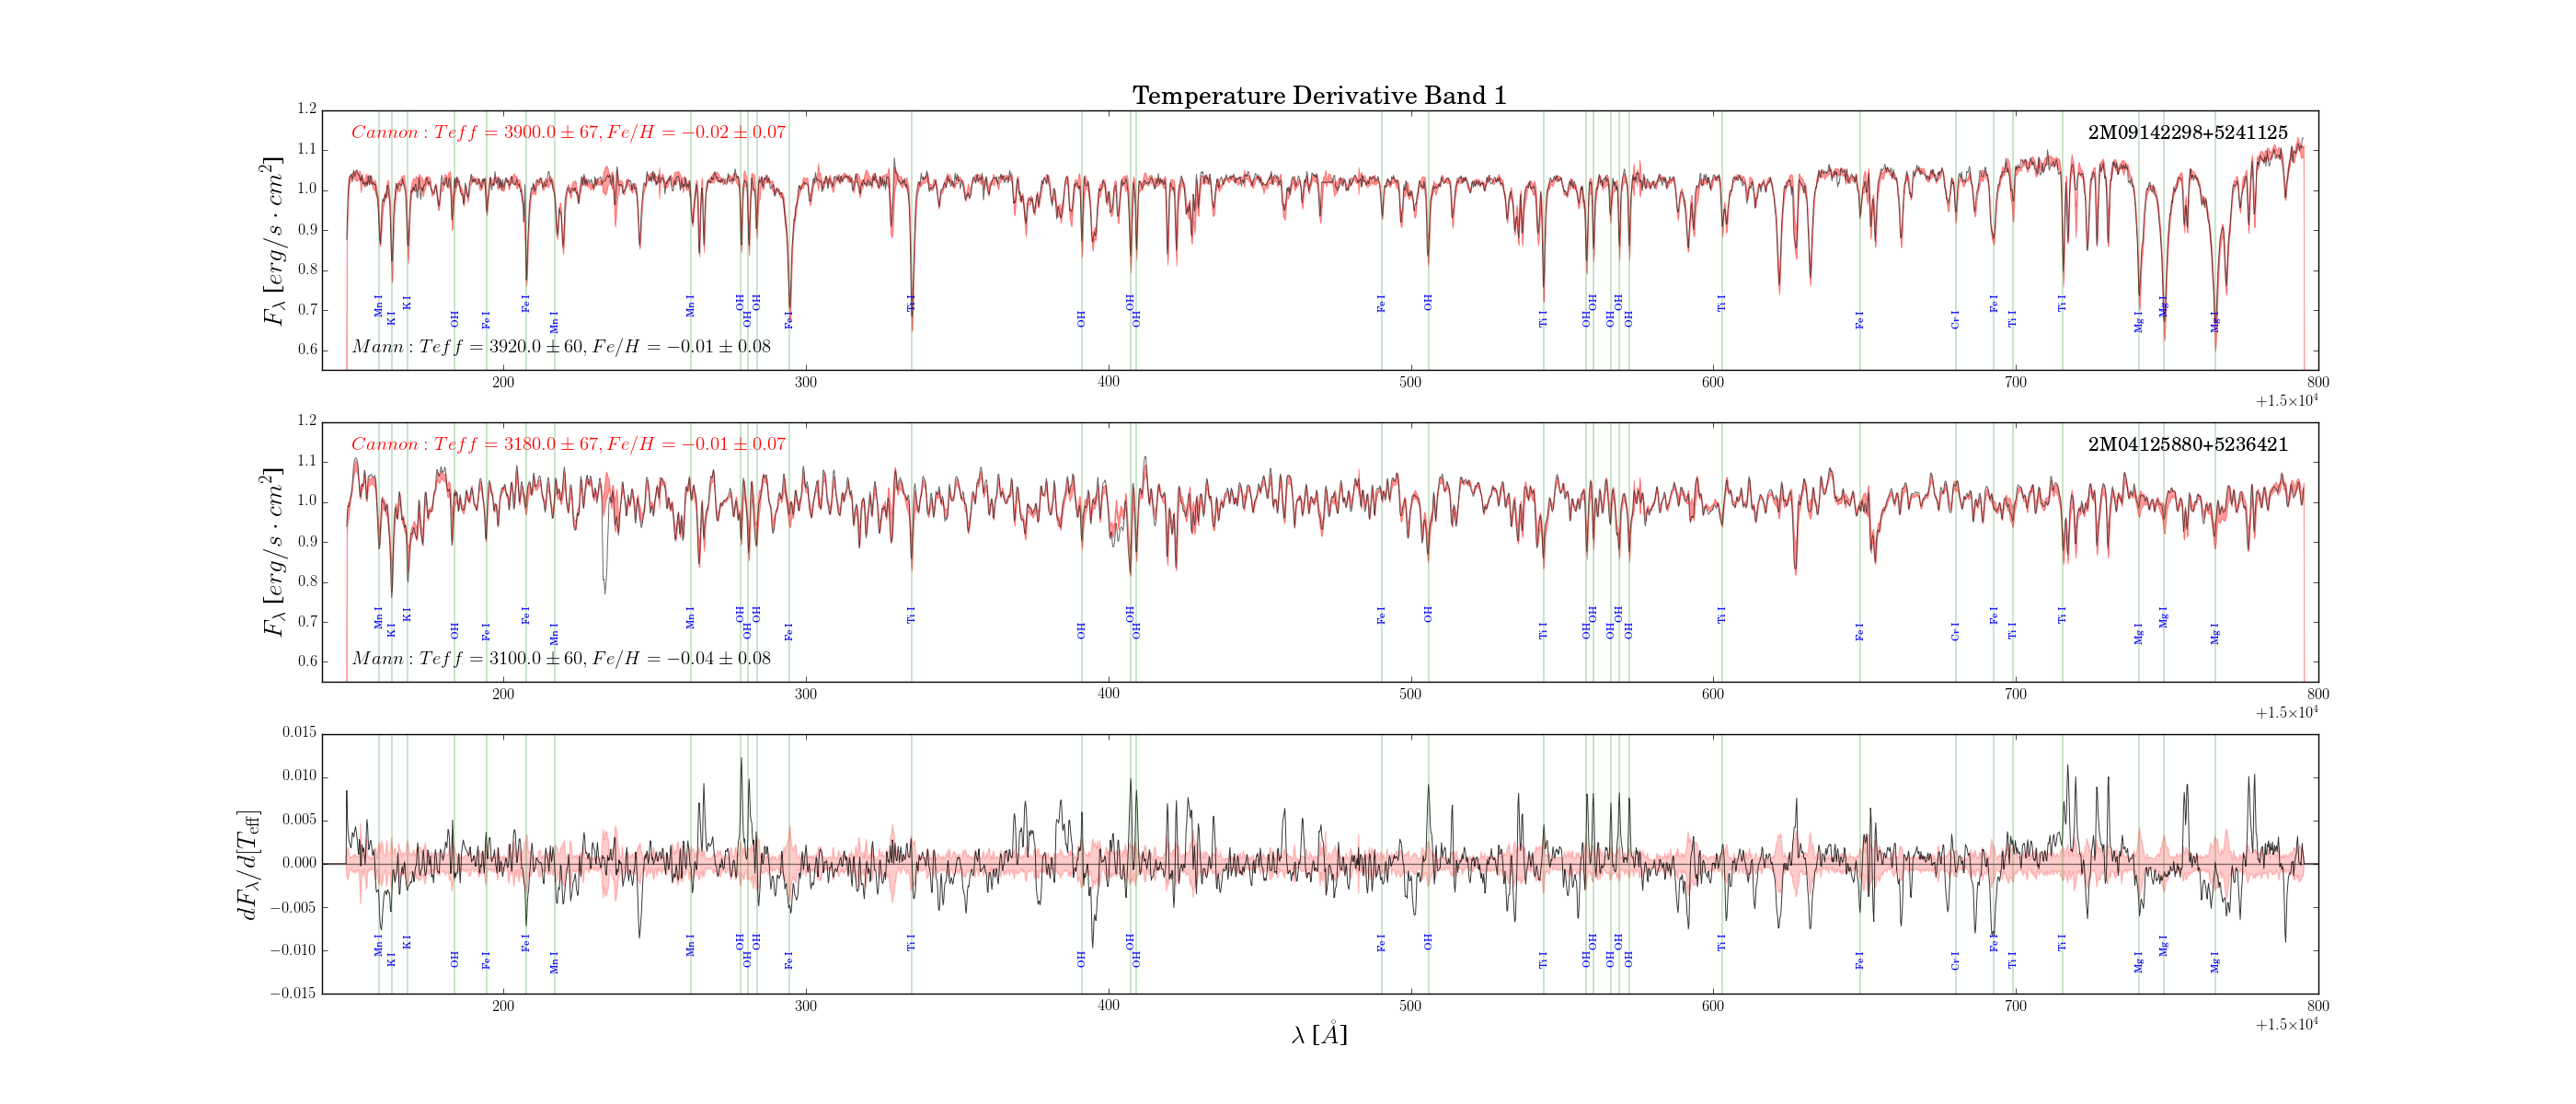
\includegraphics[width=16cm]{figures/demo_derivatives_teff1.png}
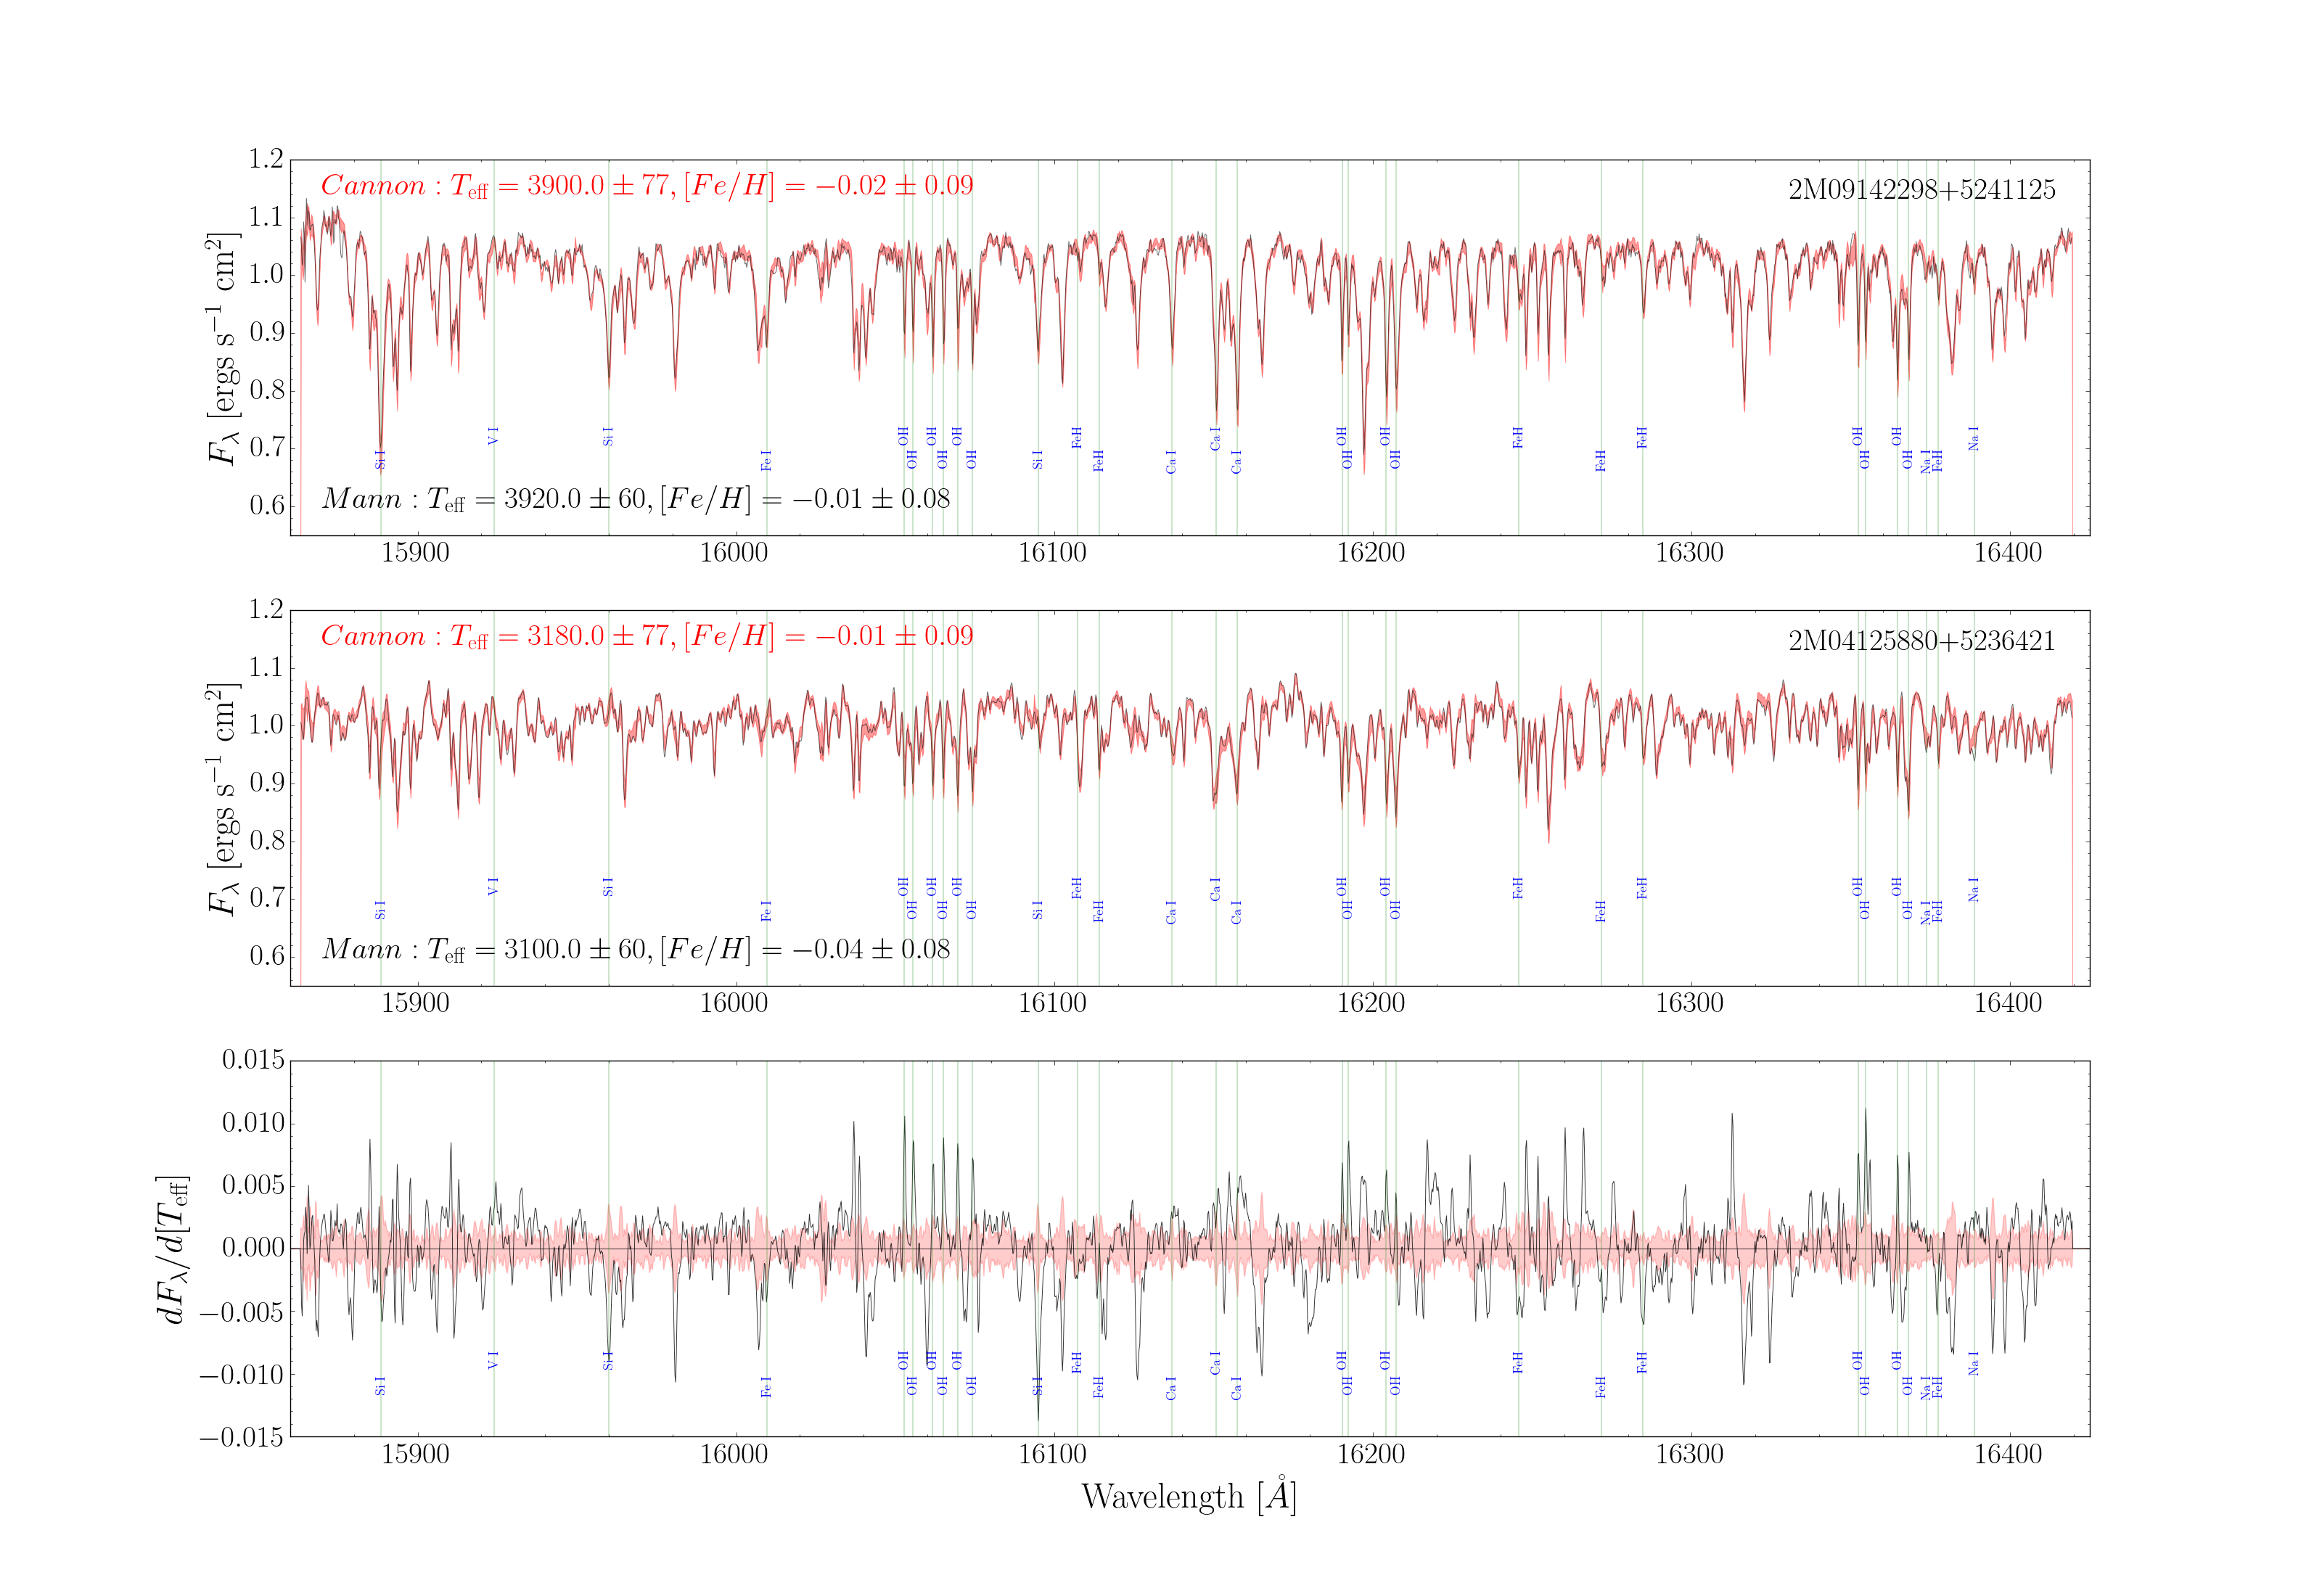
\includegraphics[width=16cm]{figures/demo_derivatives_teff2.png}
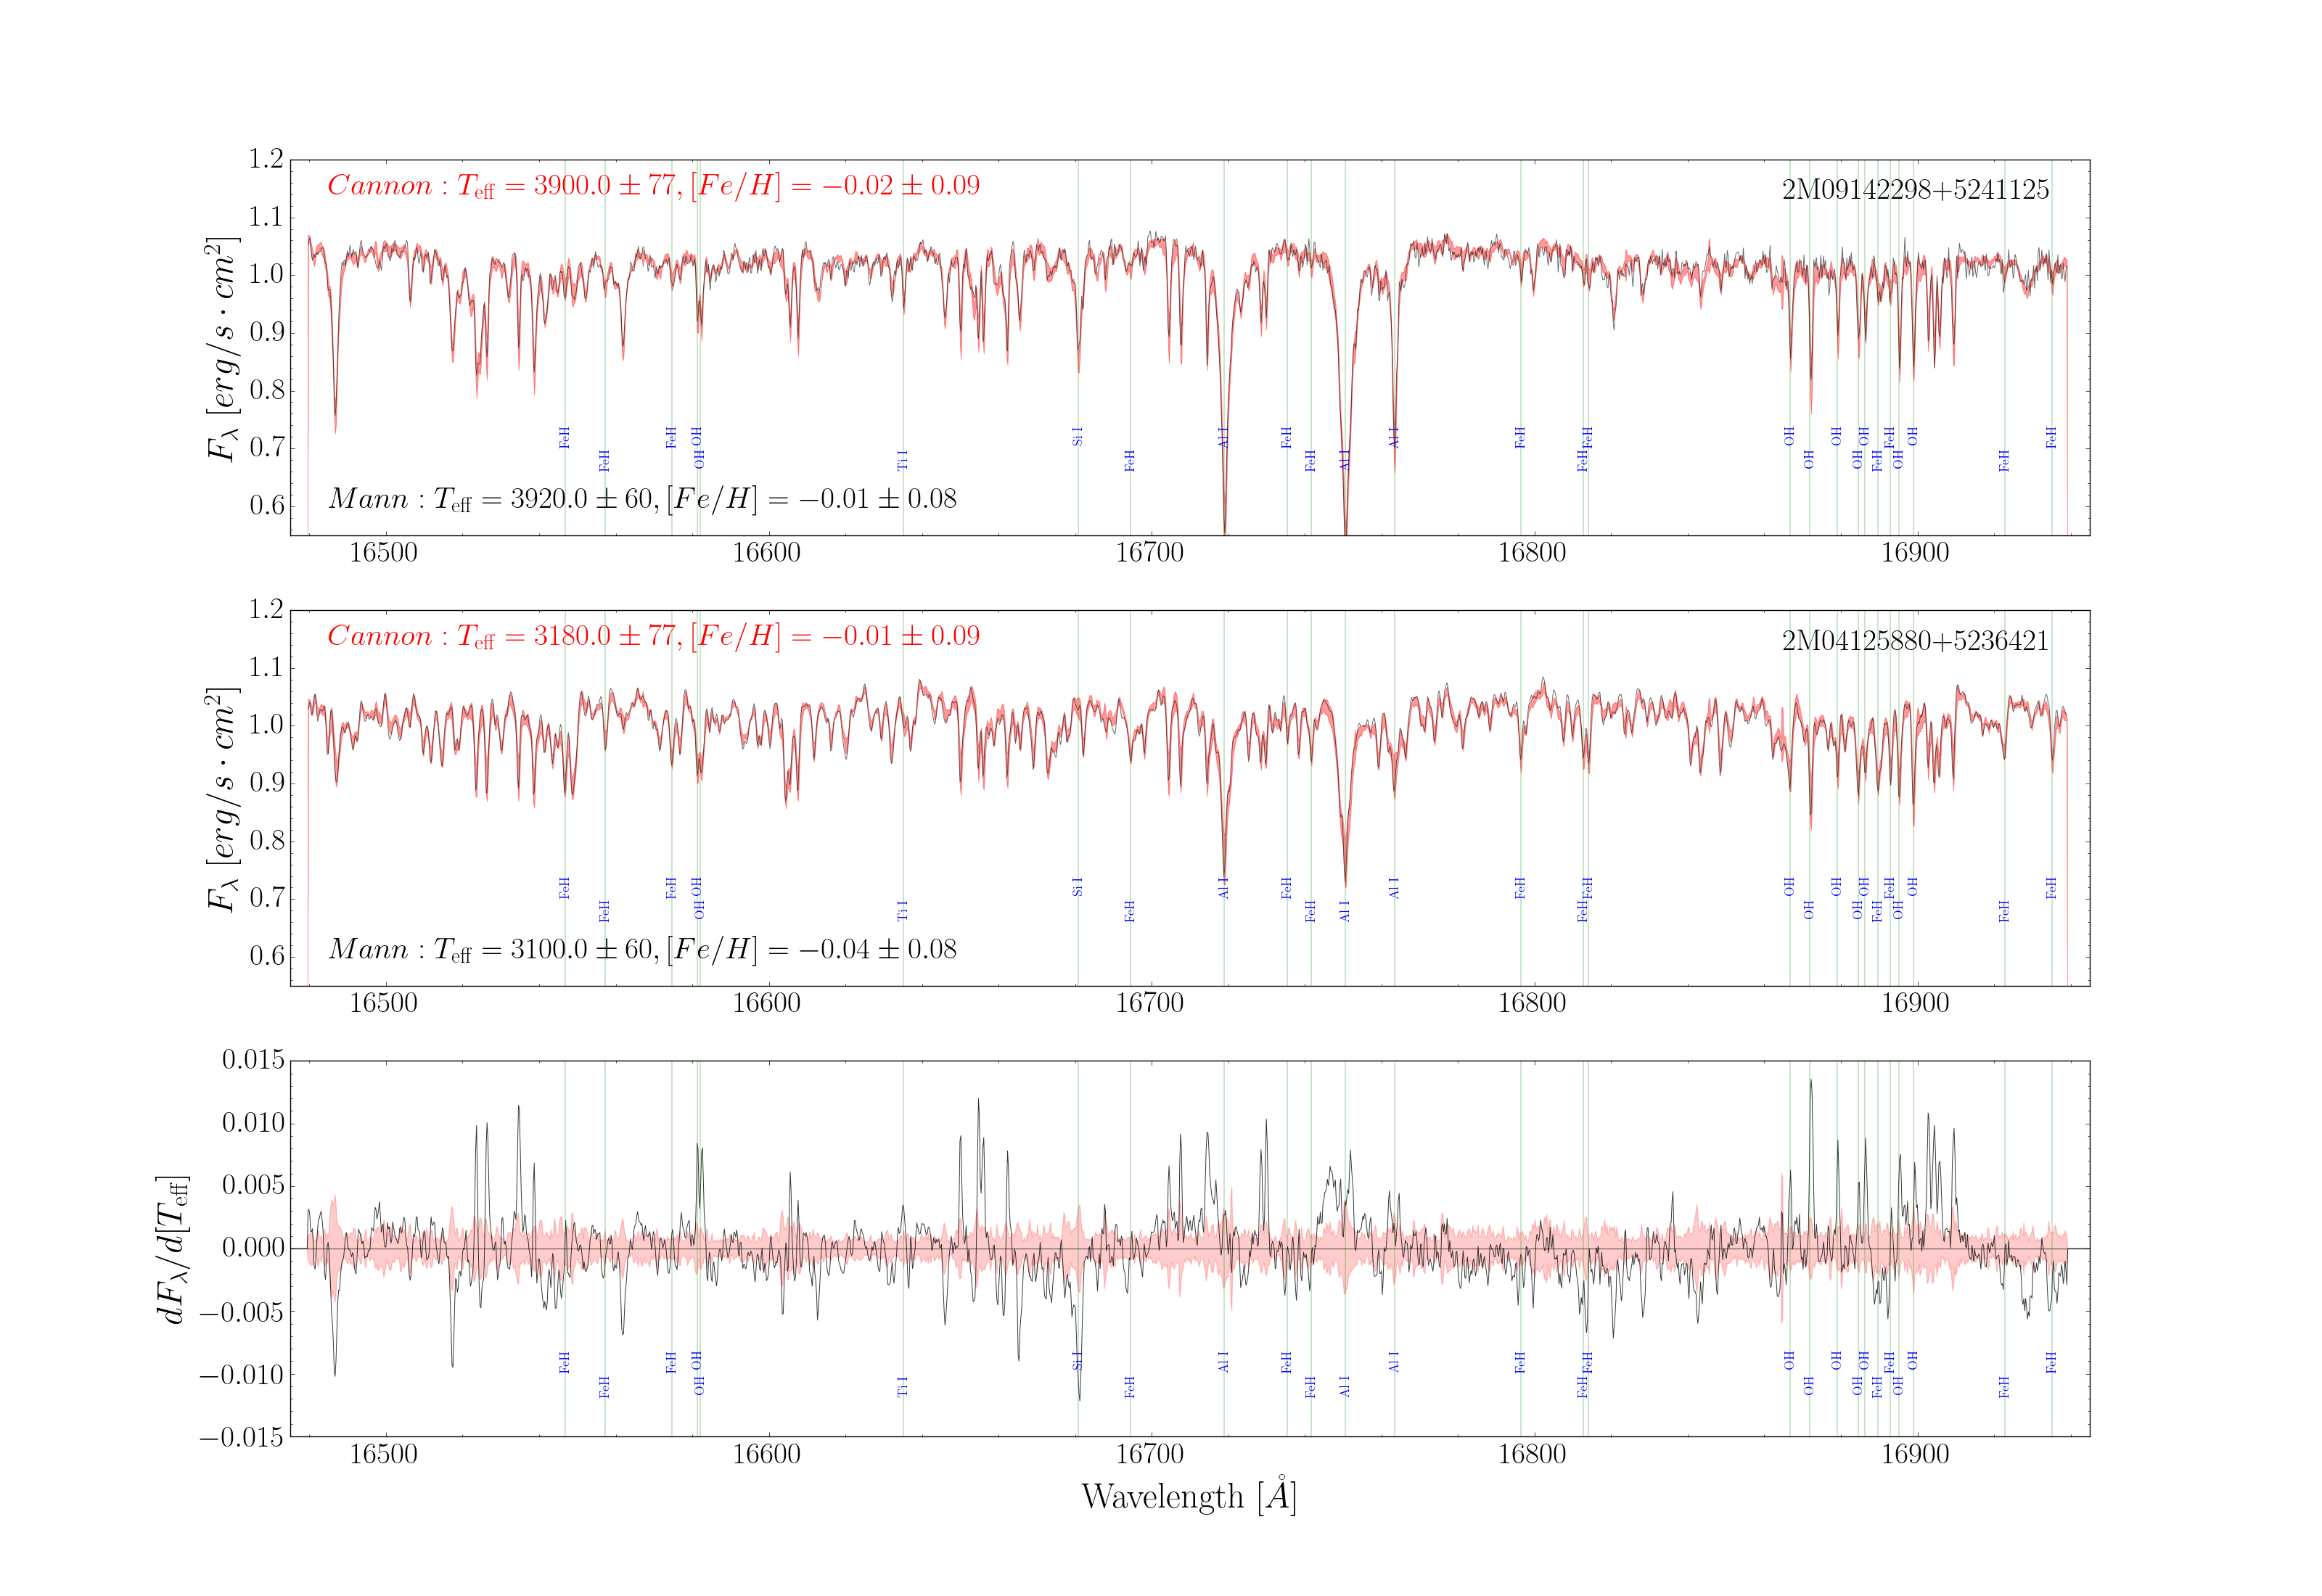
\includegraphics[width=16cm]{figures/demo_derivatives_teff3.png}
\end{center}
\caption{\textit{Top two panels of each plot:} Mann-trained model for varying temperatures, and similar metallcities. \textit{Third panel of each plot:} Derivative of \thecannon\ model with respect to temperature, taken at the median training temperature, T$_{\rm eff}=3463 K$}. \label{fig:demo_teff}
\end{figure}

%---------------------------
\begin{figure}[ht]
\begin{center}
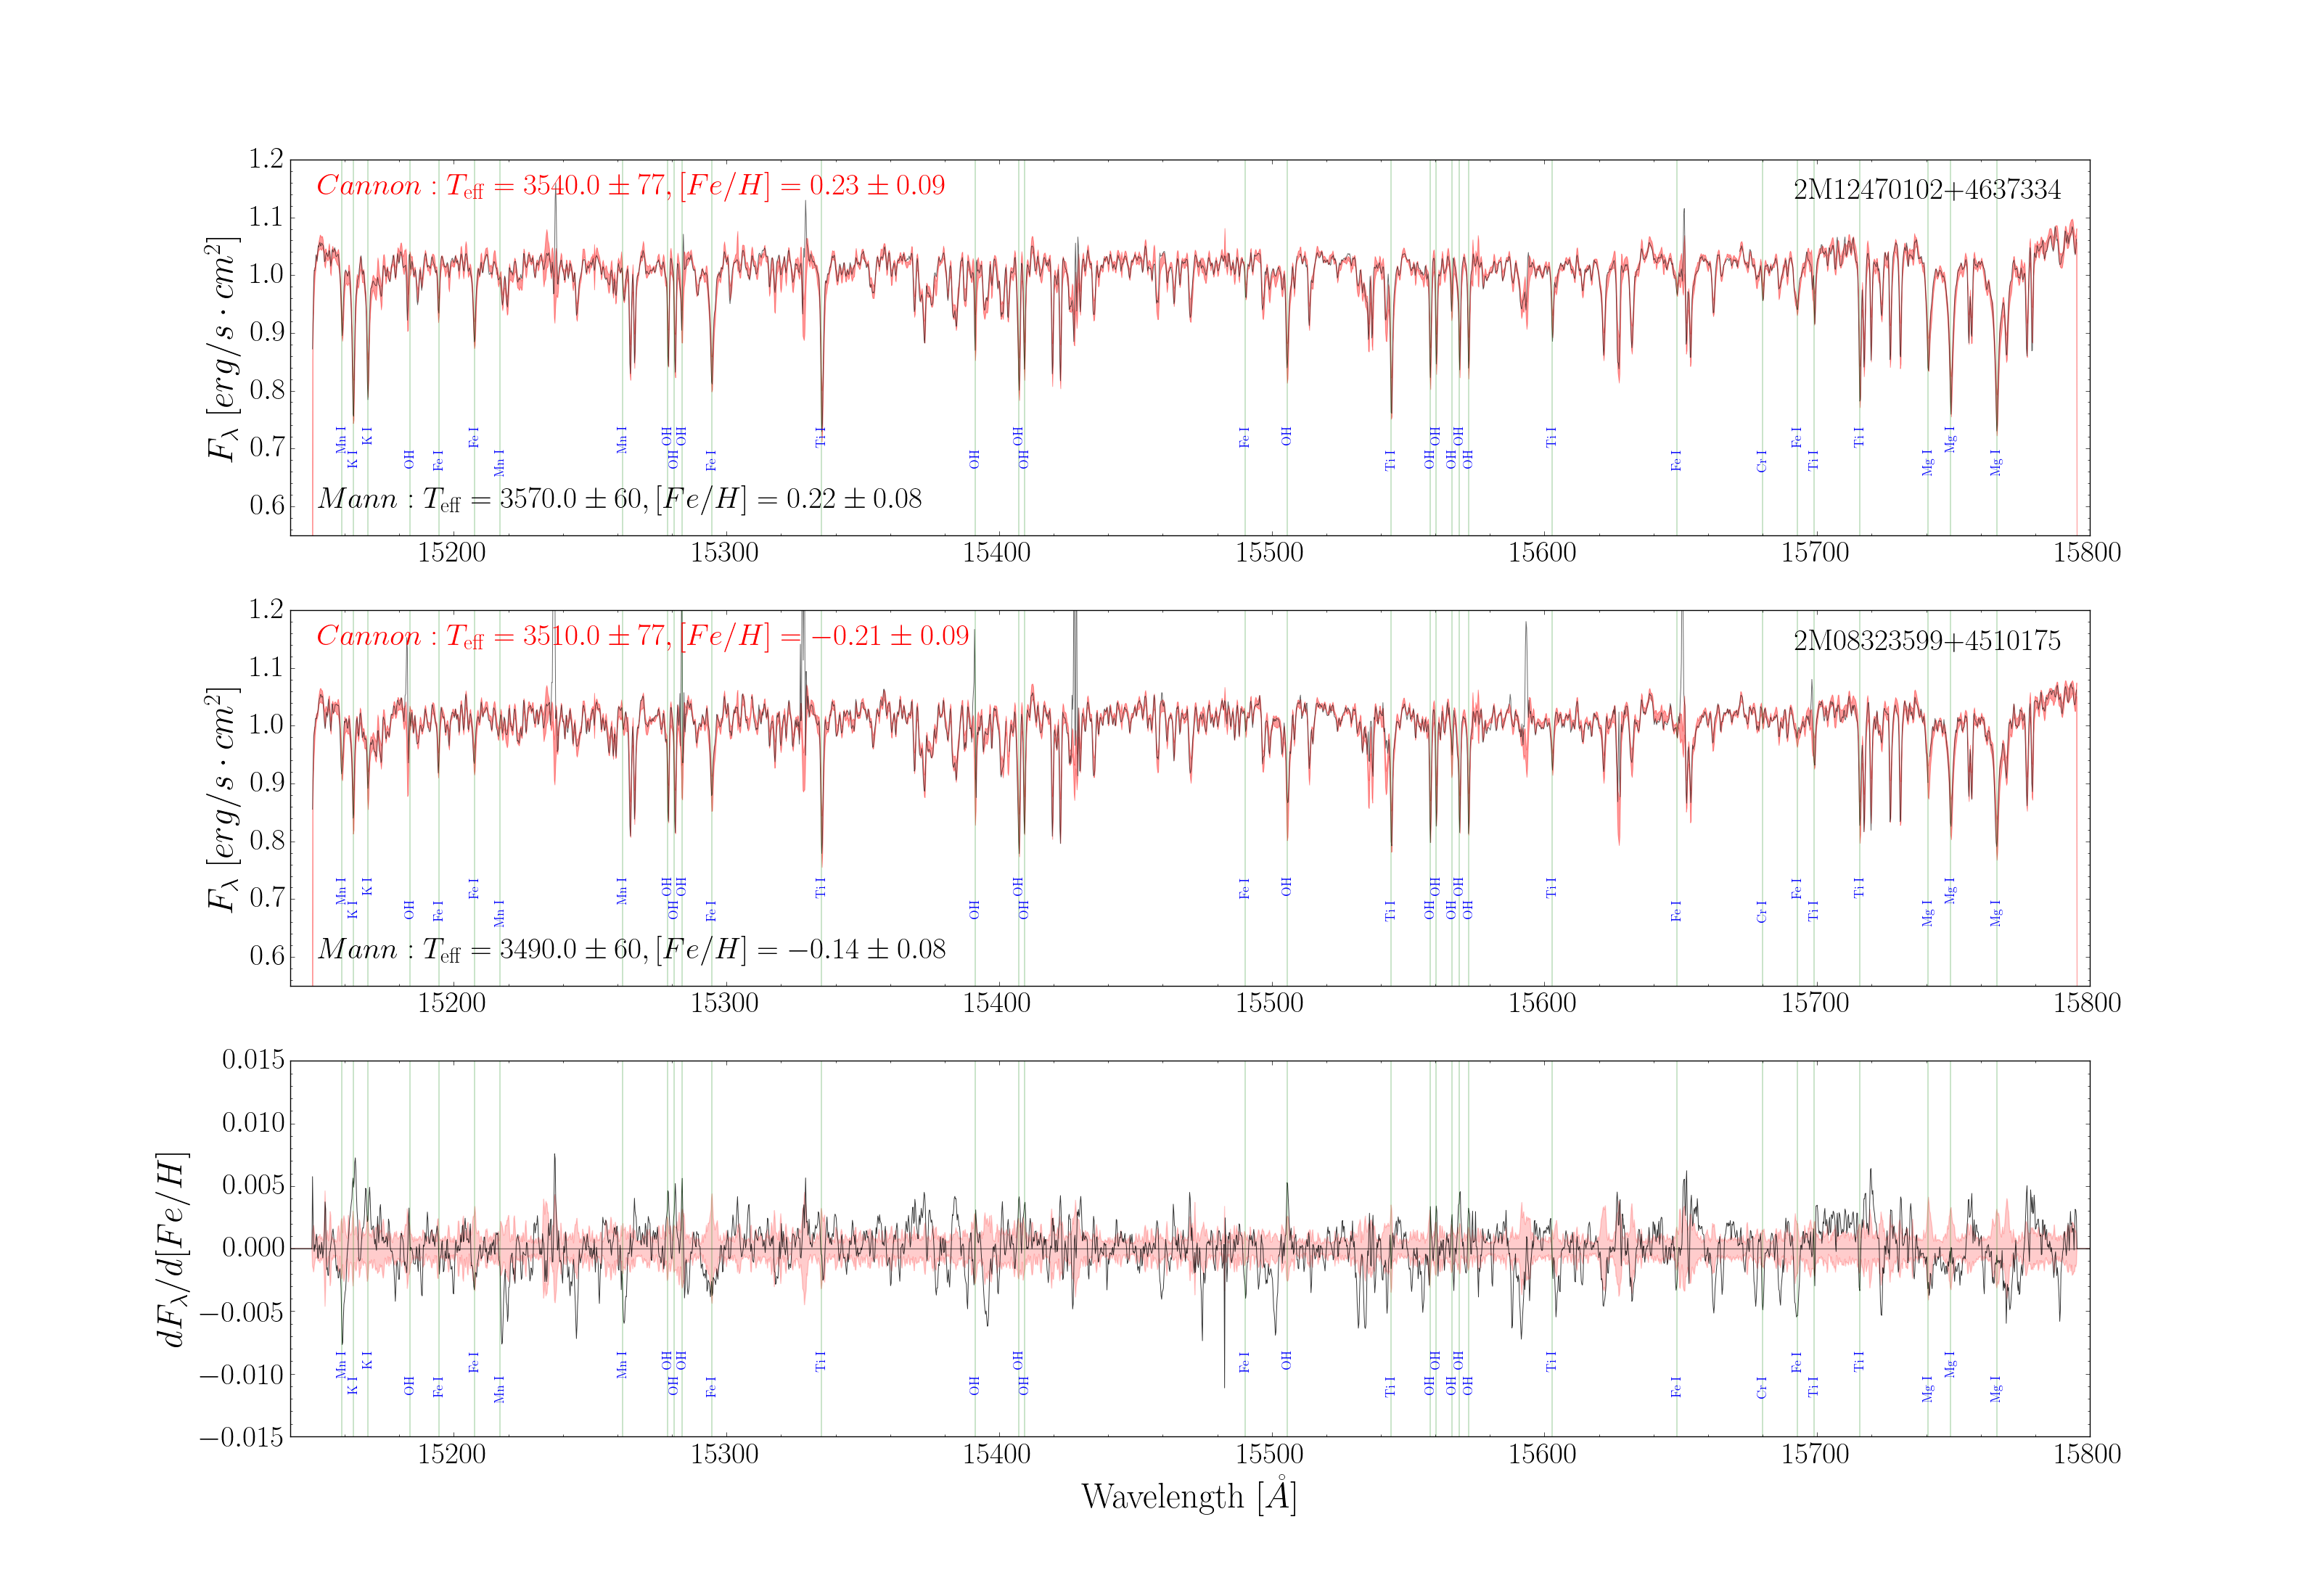
\includegraphics[width=16cm]{figures/demo_derivatives_feh1.png}
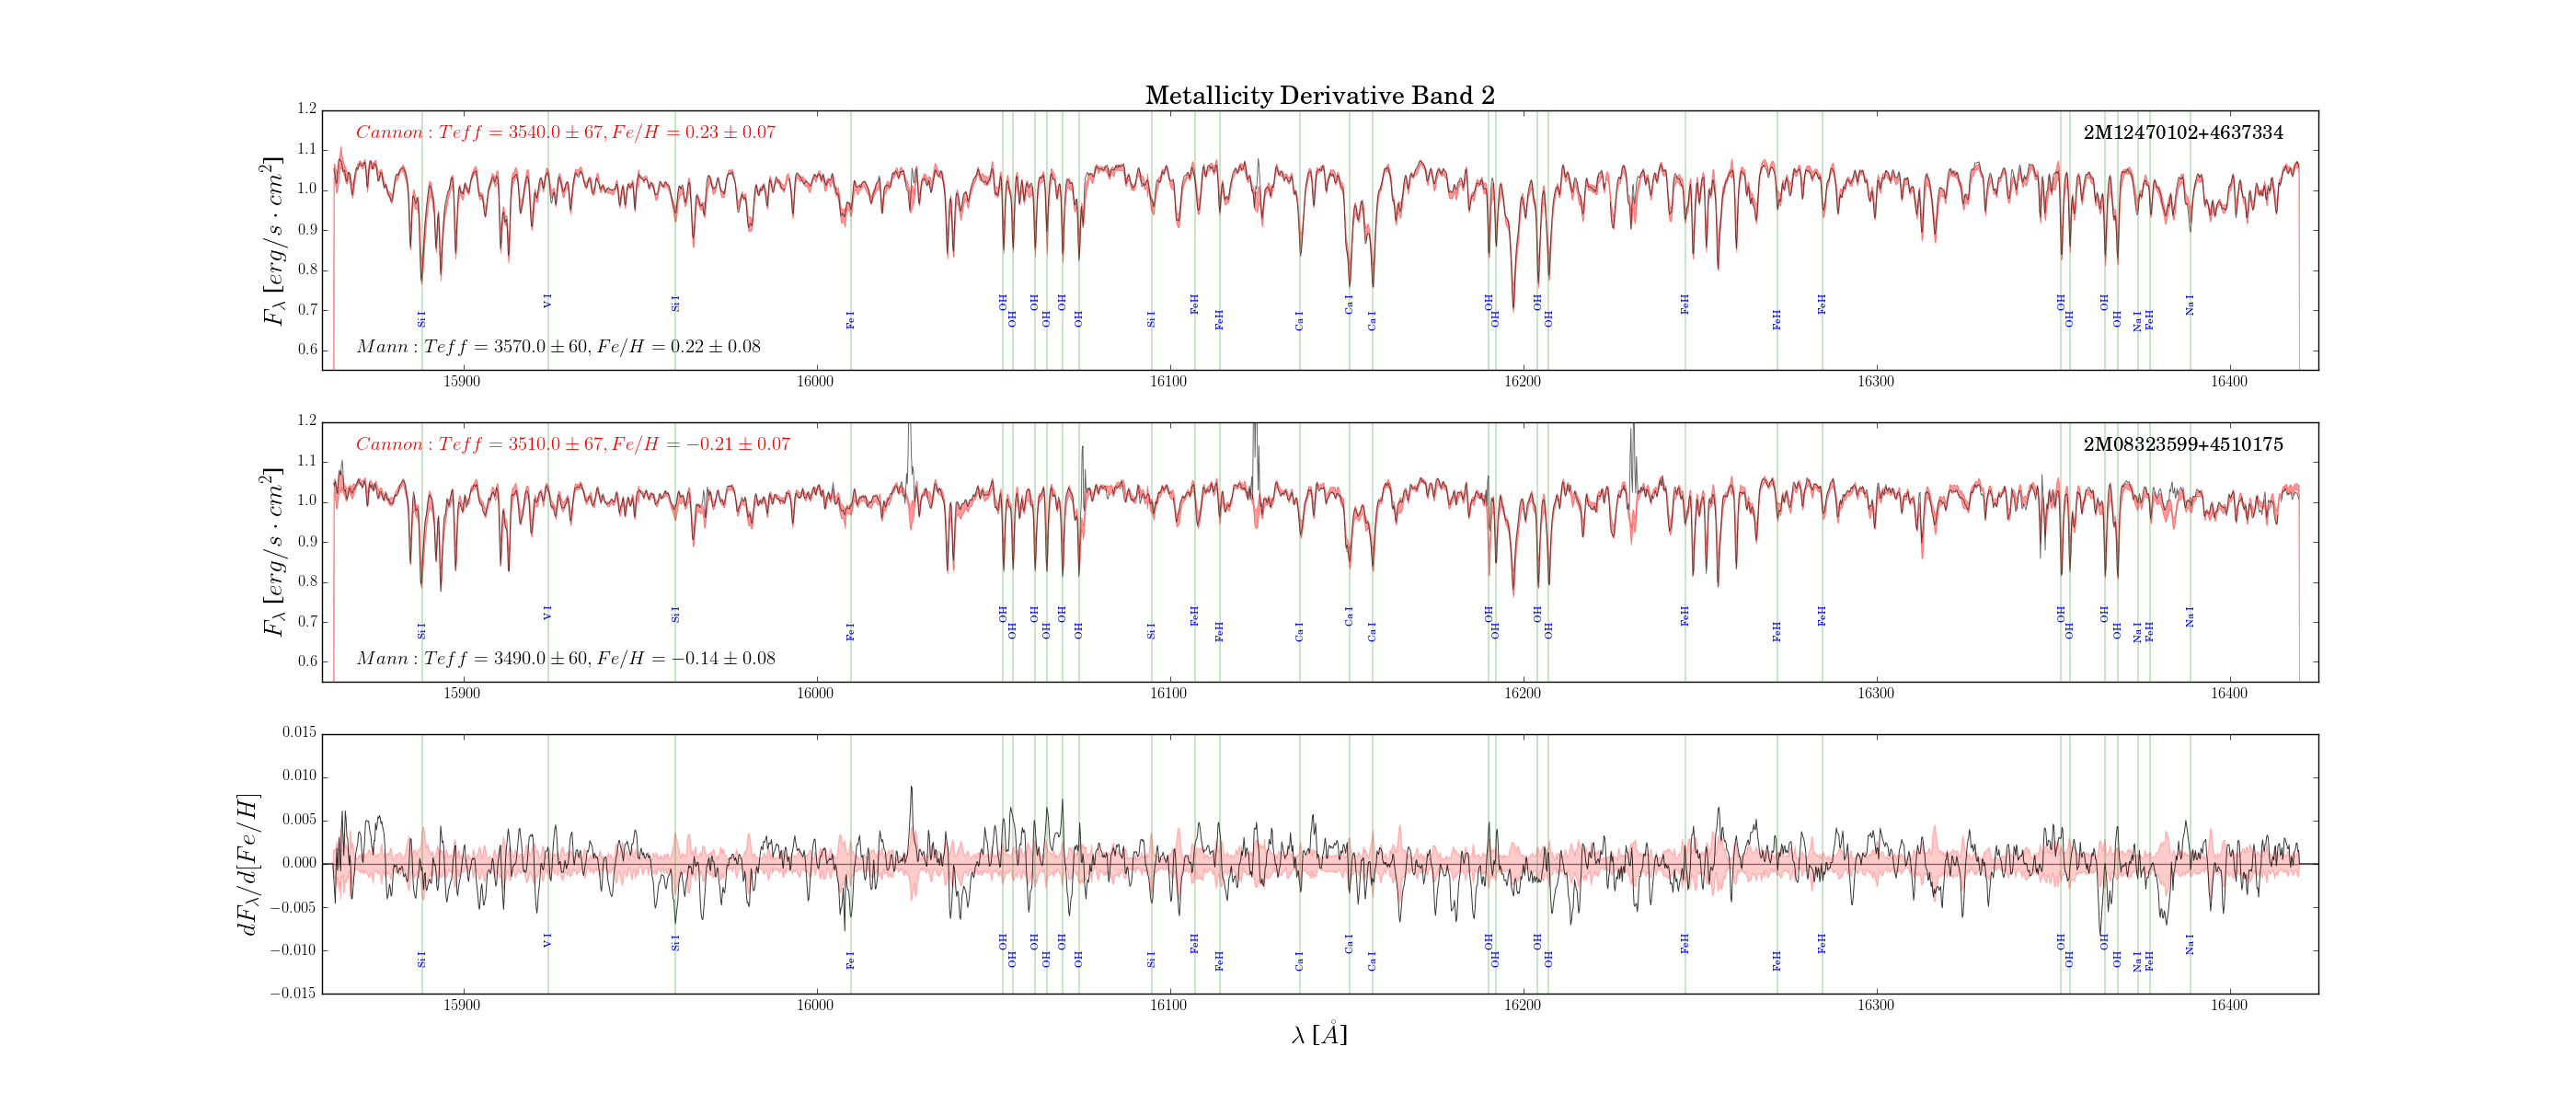
\includegraphics[width=16cm]{figures/demo_derivatives_feh2.png}
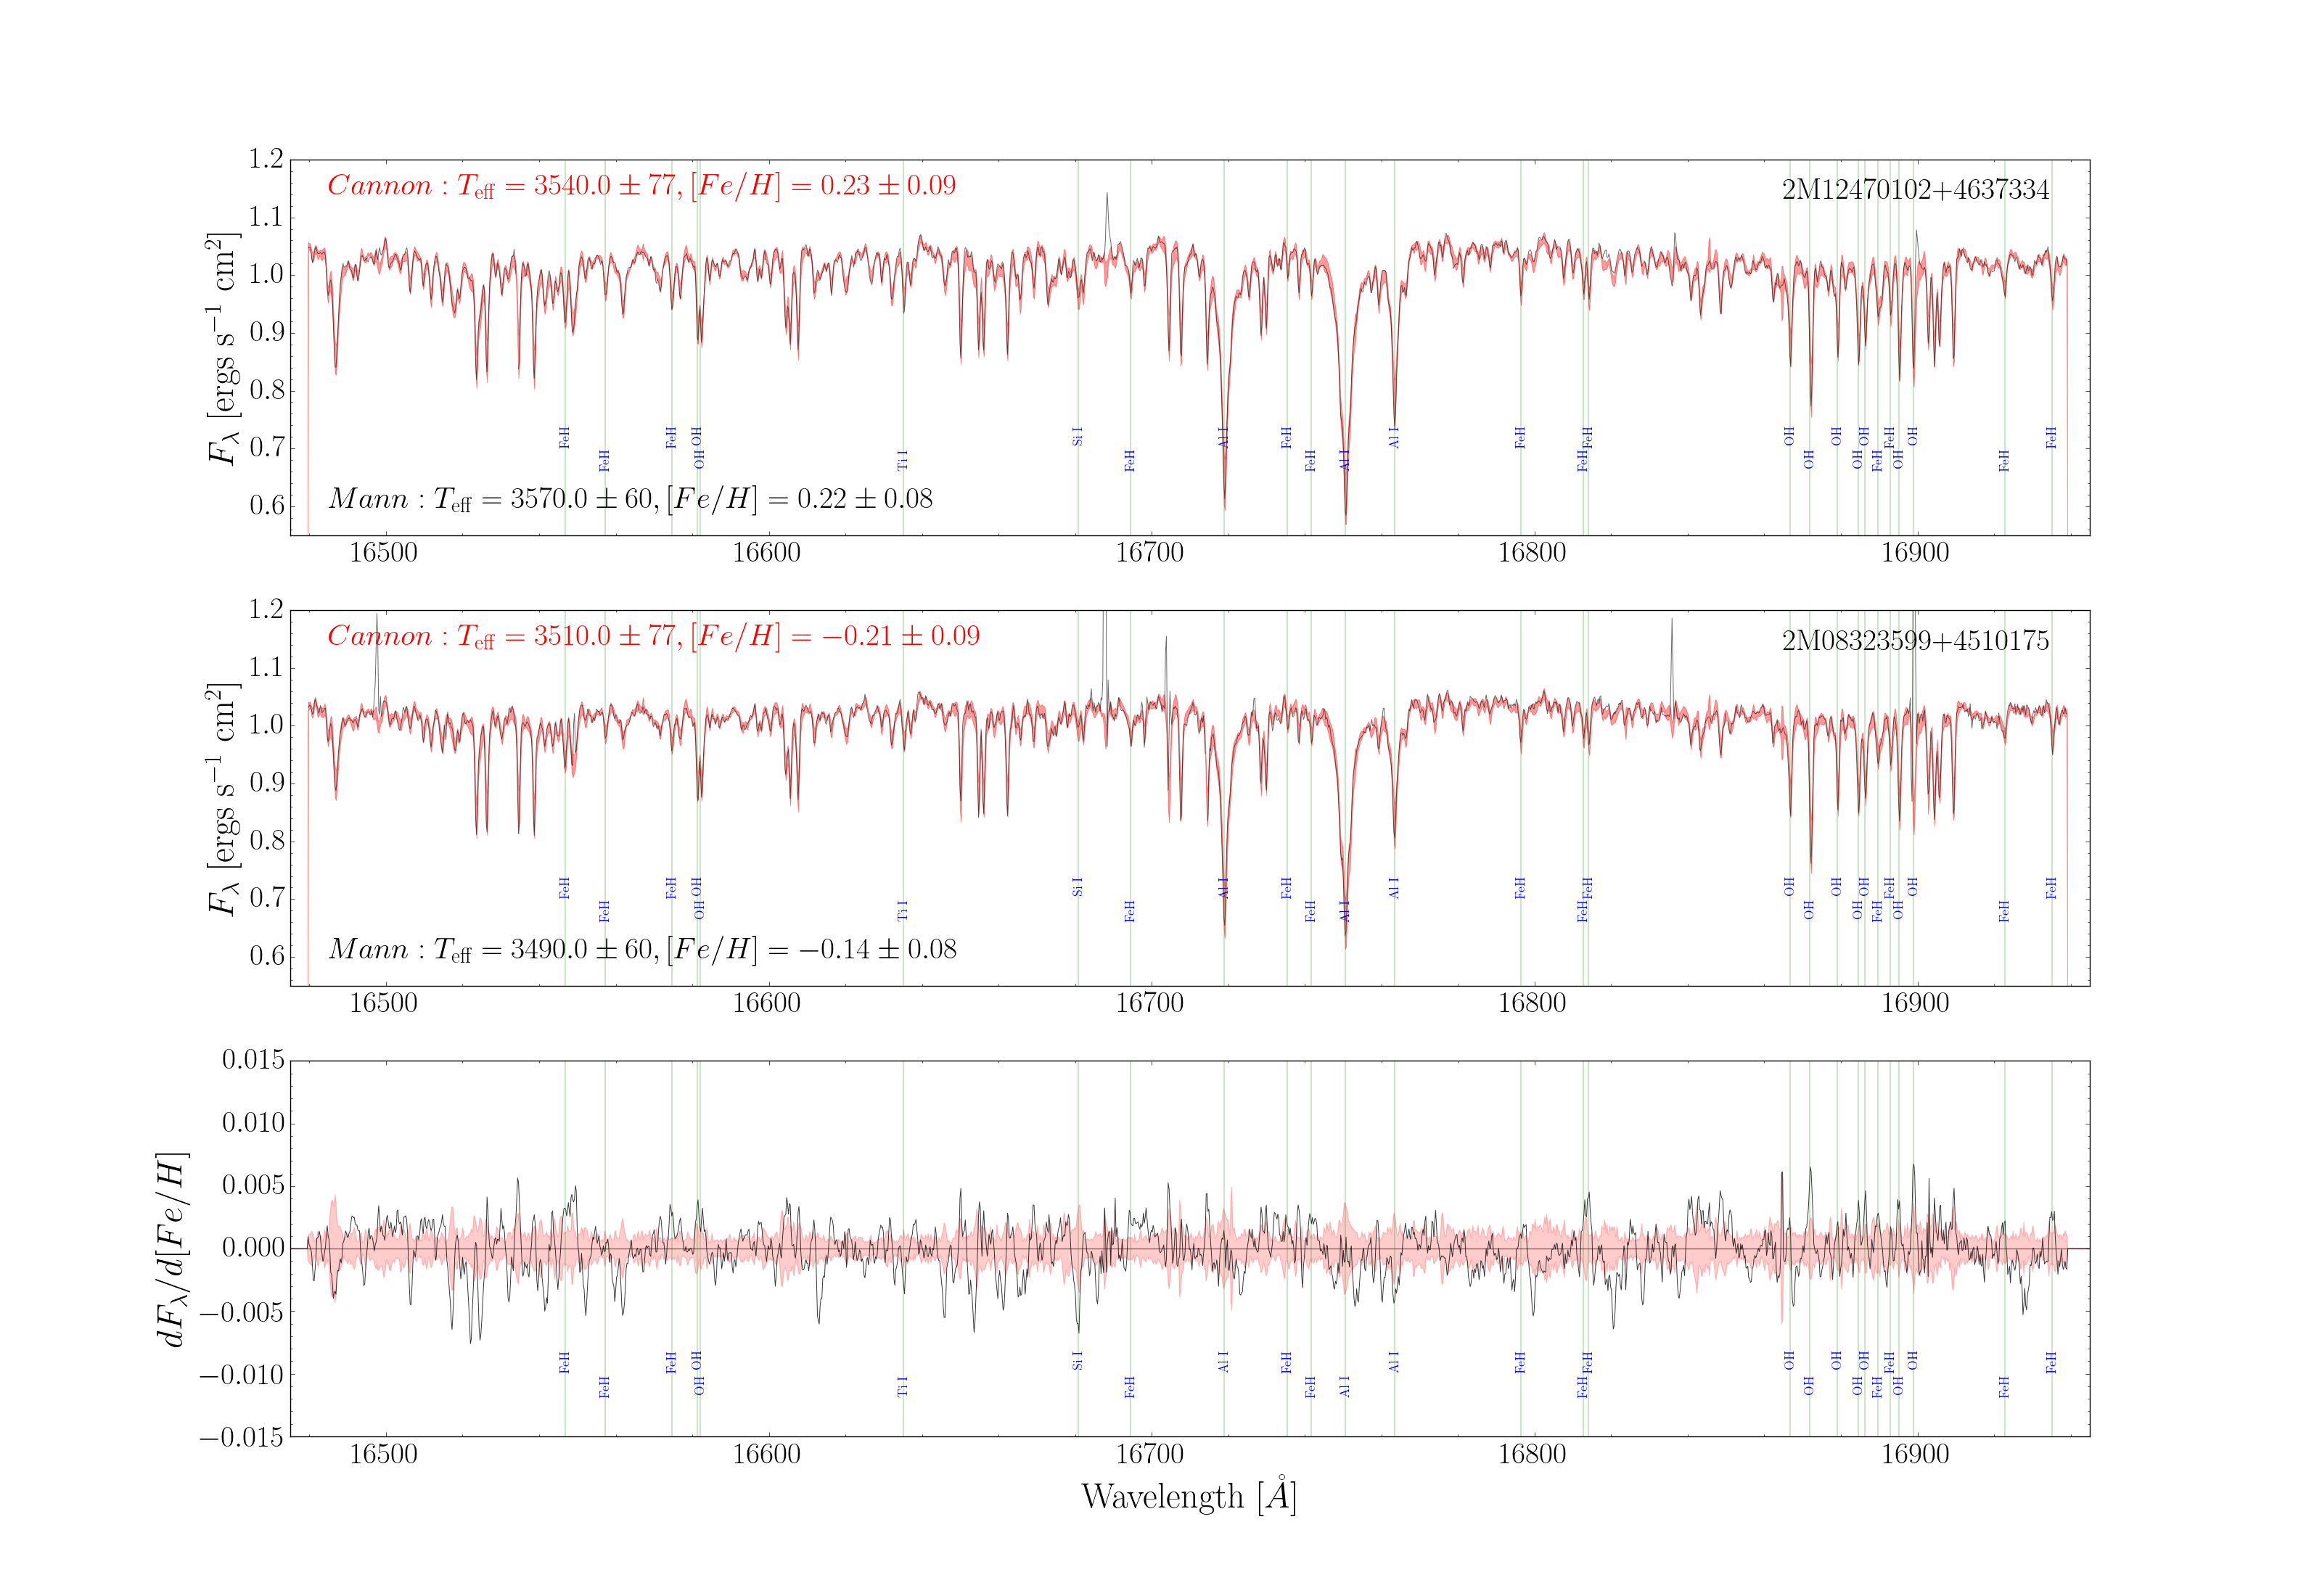
\includegraphics[width=16cm]{figures/demo_derivatives_feh3.png}
\end{center}
\caption{\textit{Top two panels of each plot:} Mann-trained model for varying metallicities and similar temperatures. \textit{Third panel:} Derivative of \thecannon\ model with respect to metallicity, taken at the median training metallicity, [Fe/H]$=-0.03$.} \label{fig:demo_feh}
\end{figure}

%---------------------------
\begin{figure}[ht]
\begin{center}
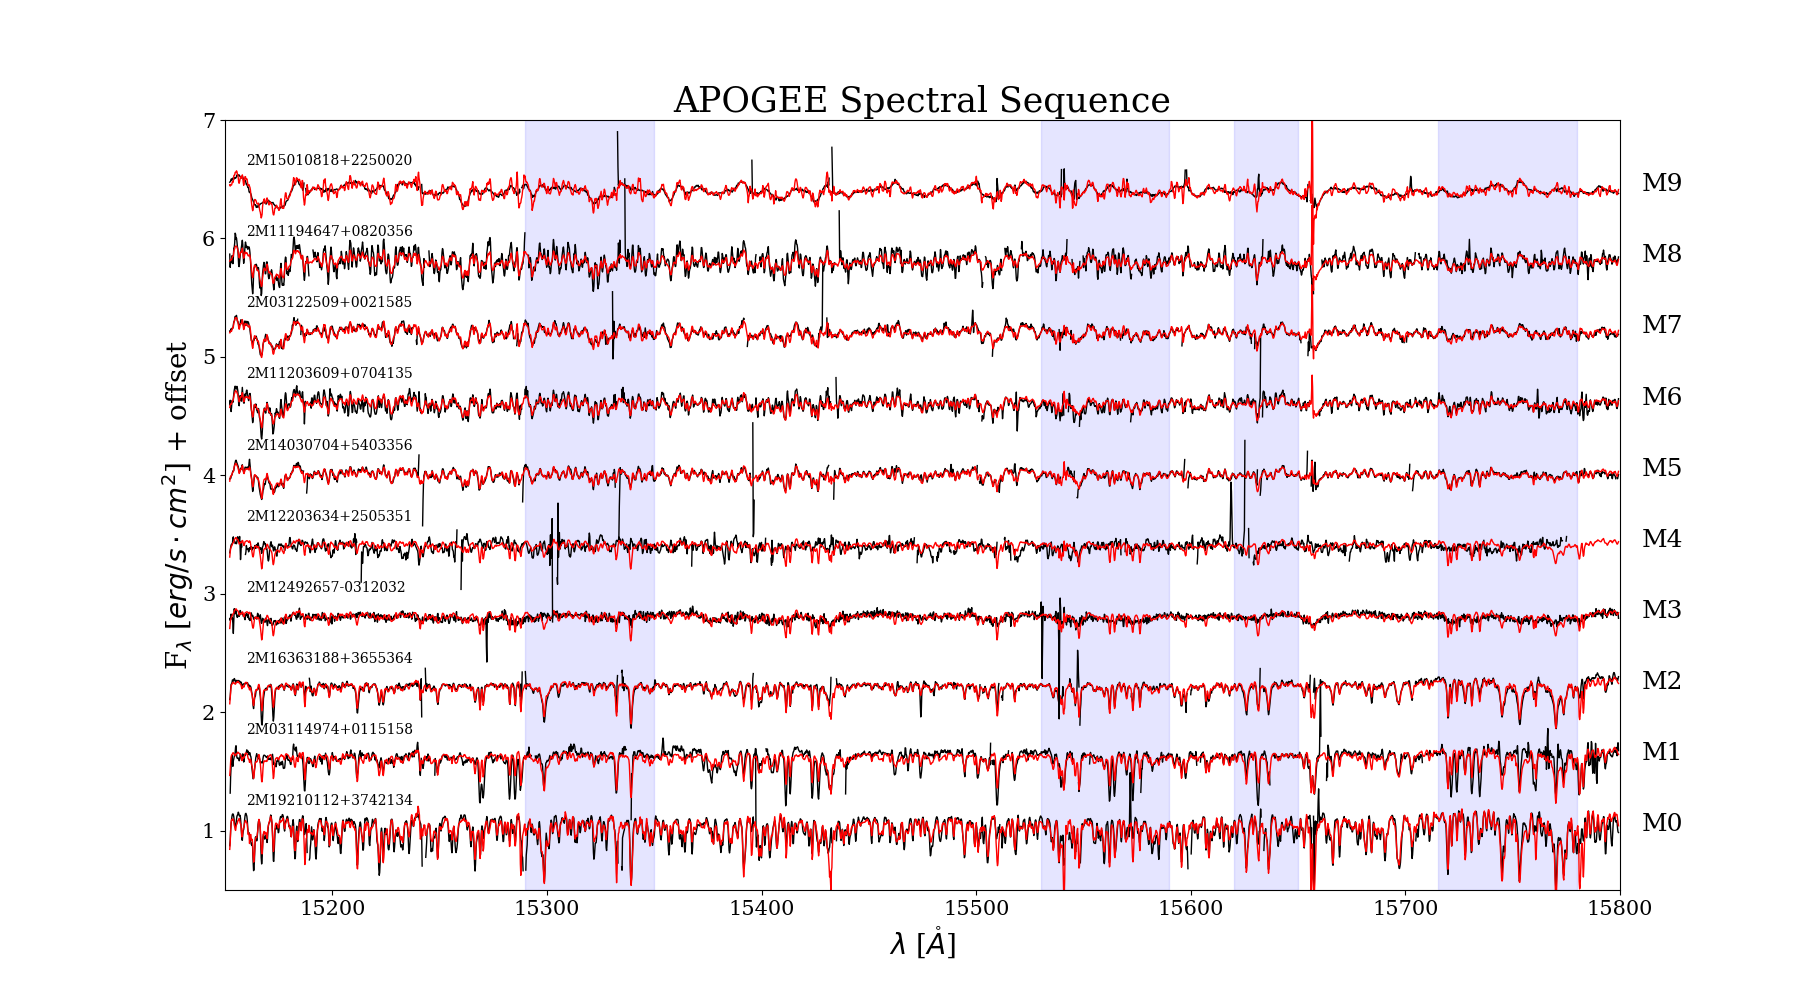
\includegraphics[width=12cm]{figures/Spectral_Sequence_1.png}
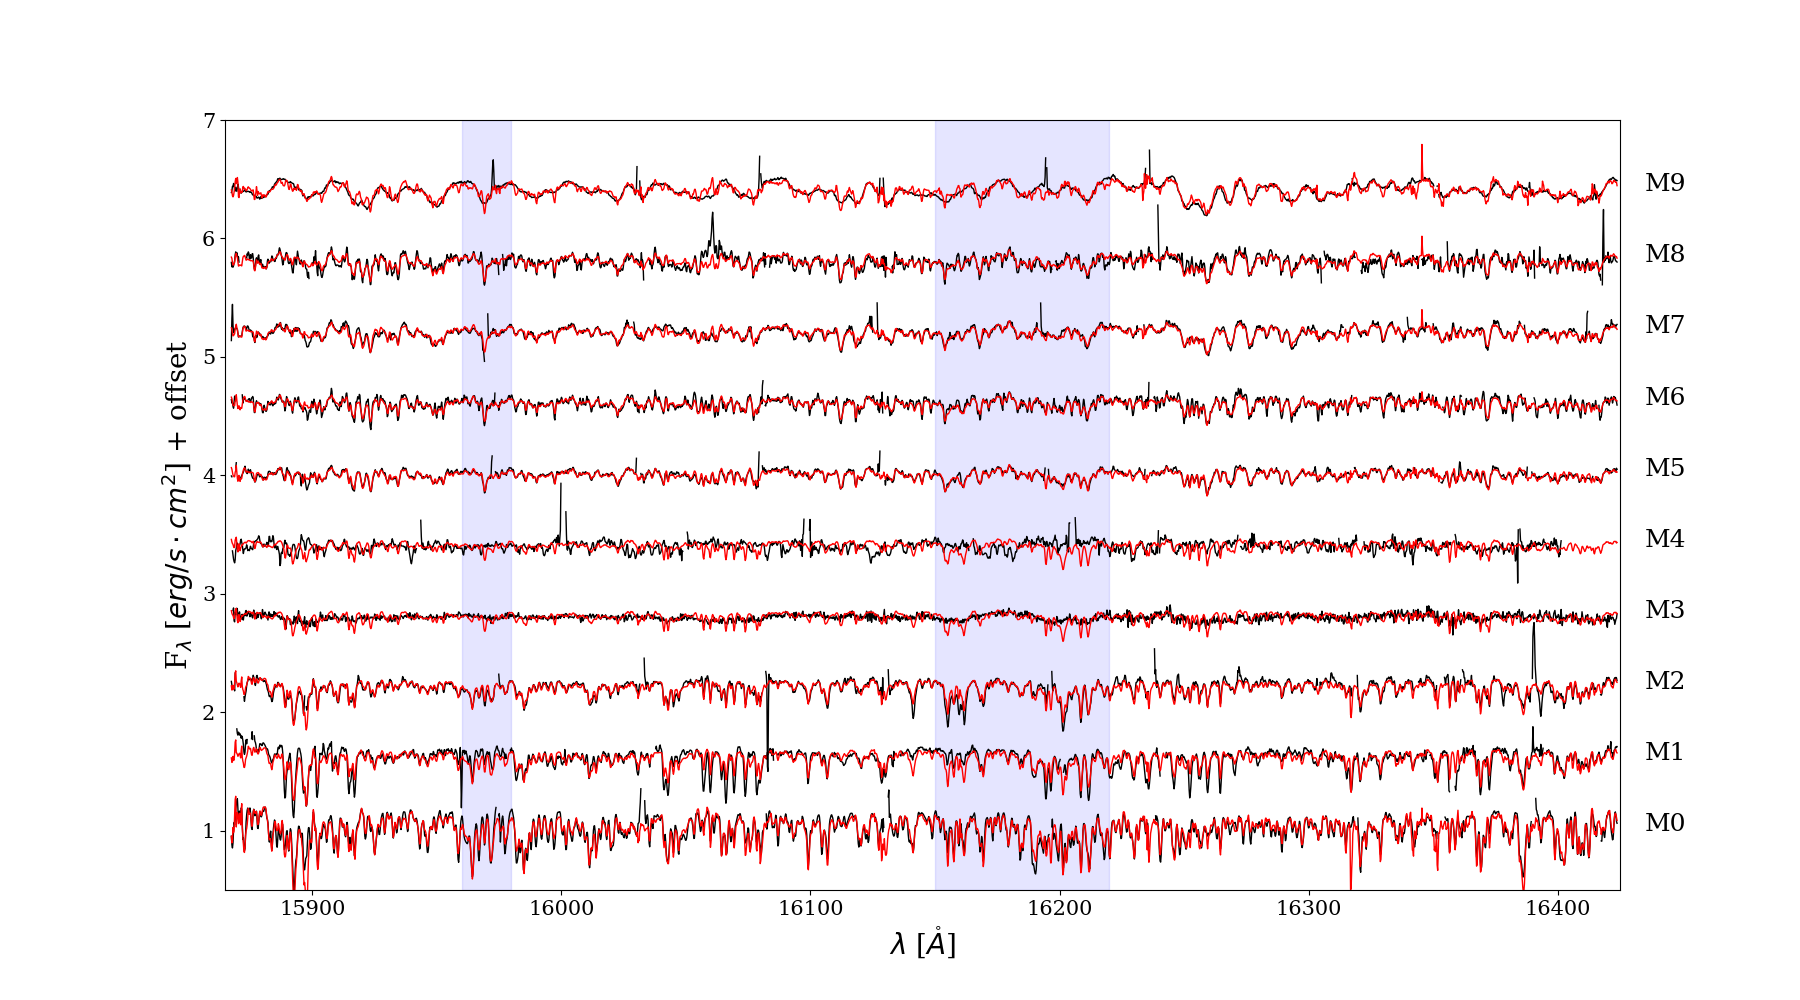
\includegraphics[width=12cm]{figures/Spectral_Sequence_2.png}
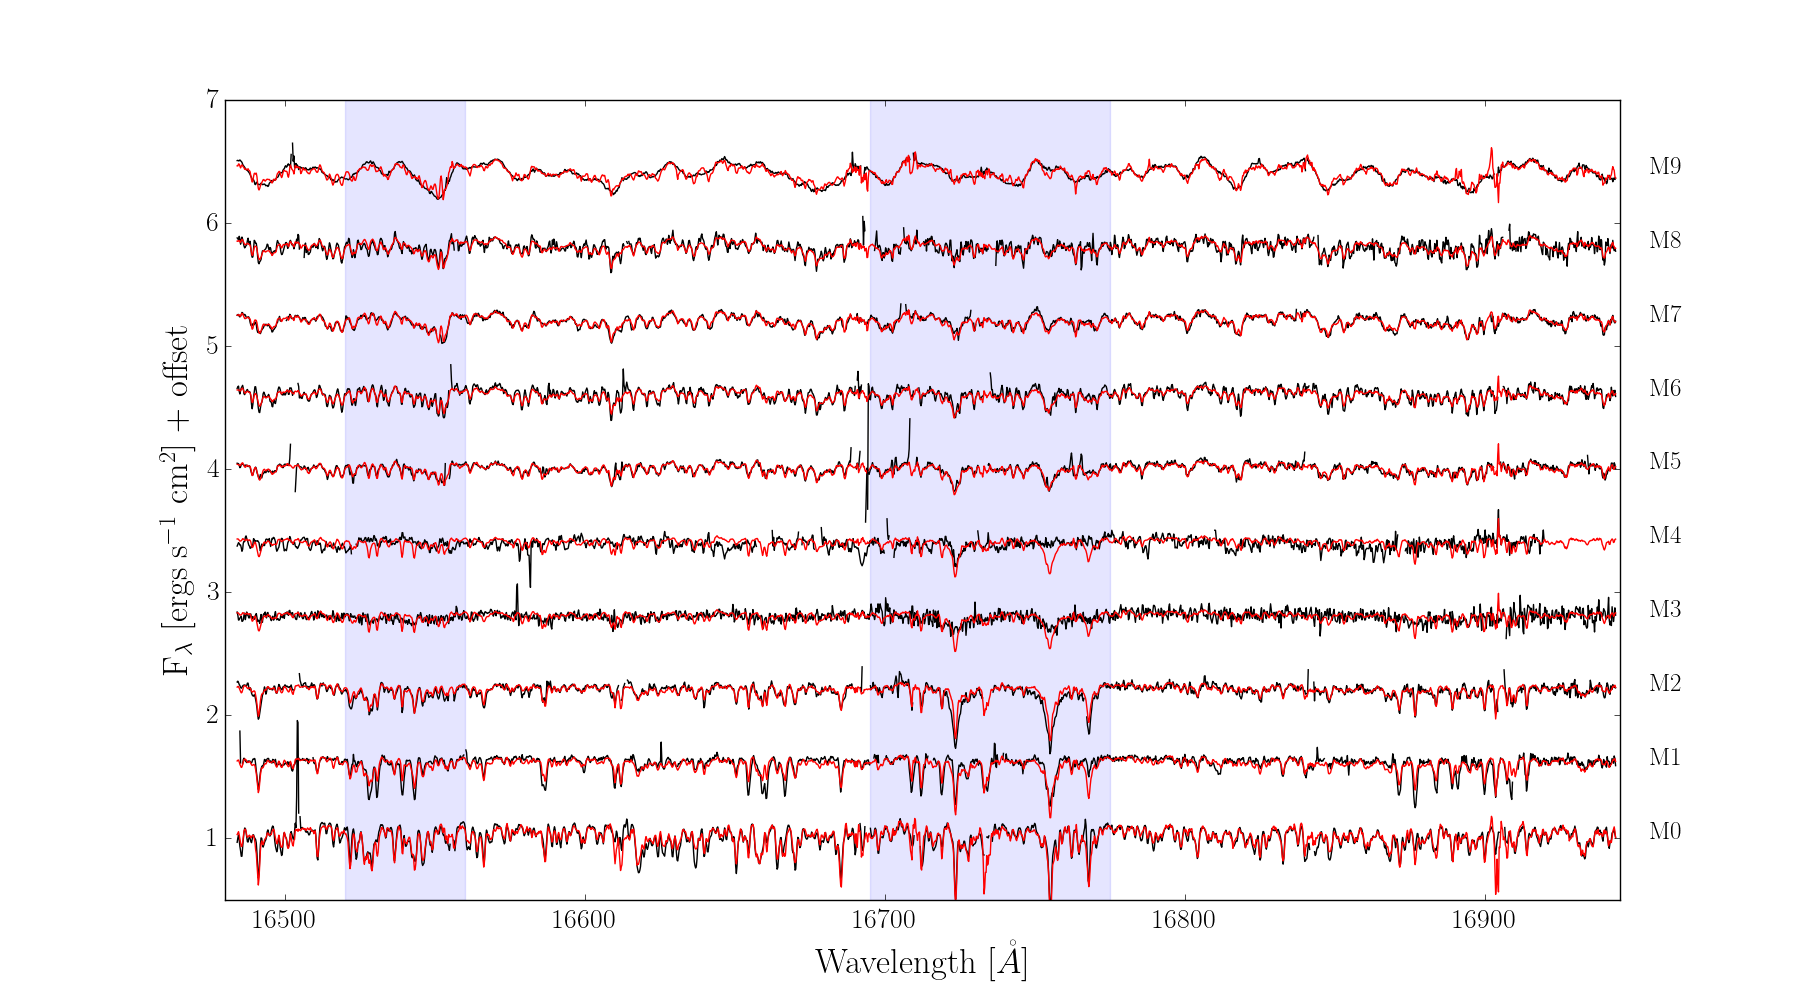
\includegraphics[width=12cm]{figures/Spectral_Sequence_3.png}
\end{center}
\caption{Spectral sequence of dwarfs in training set M0-M9; separate plots show three detector chips of \apogee\ spectrum (black), the best fit Cannon trained model (red) with highlighted spectral type sensitive regions identified in \citealt{Desphande:2013}.} \label{fig:sp_sequence}
\end{figure}

%---------------------------
\begin{figure}[ht]
\begin{center}
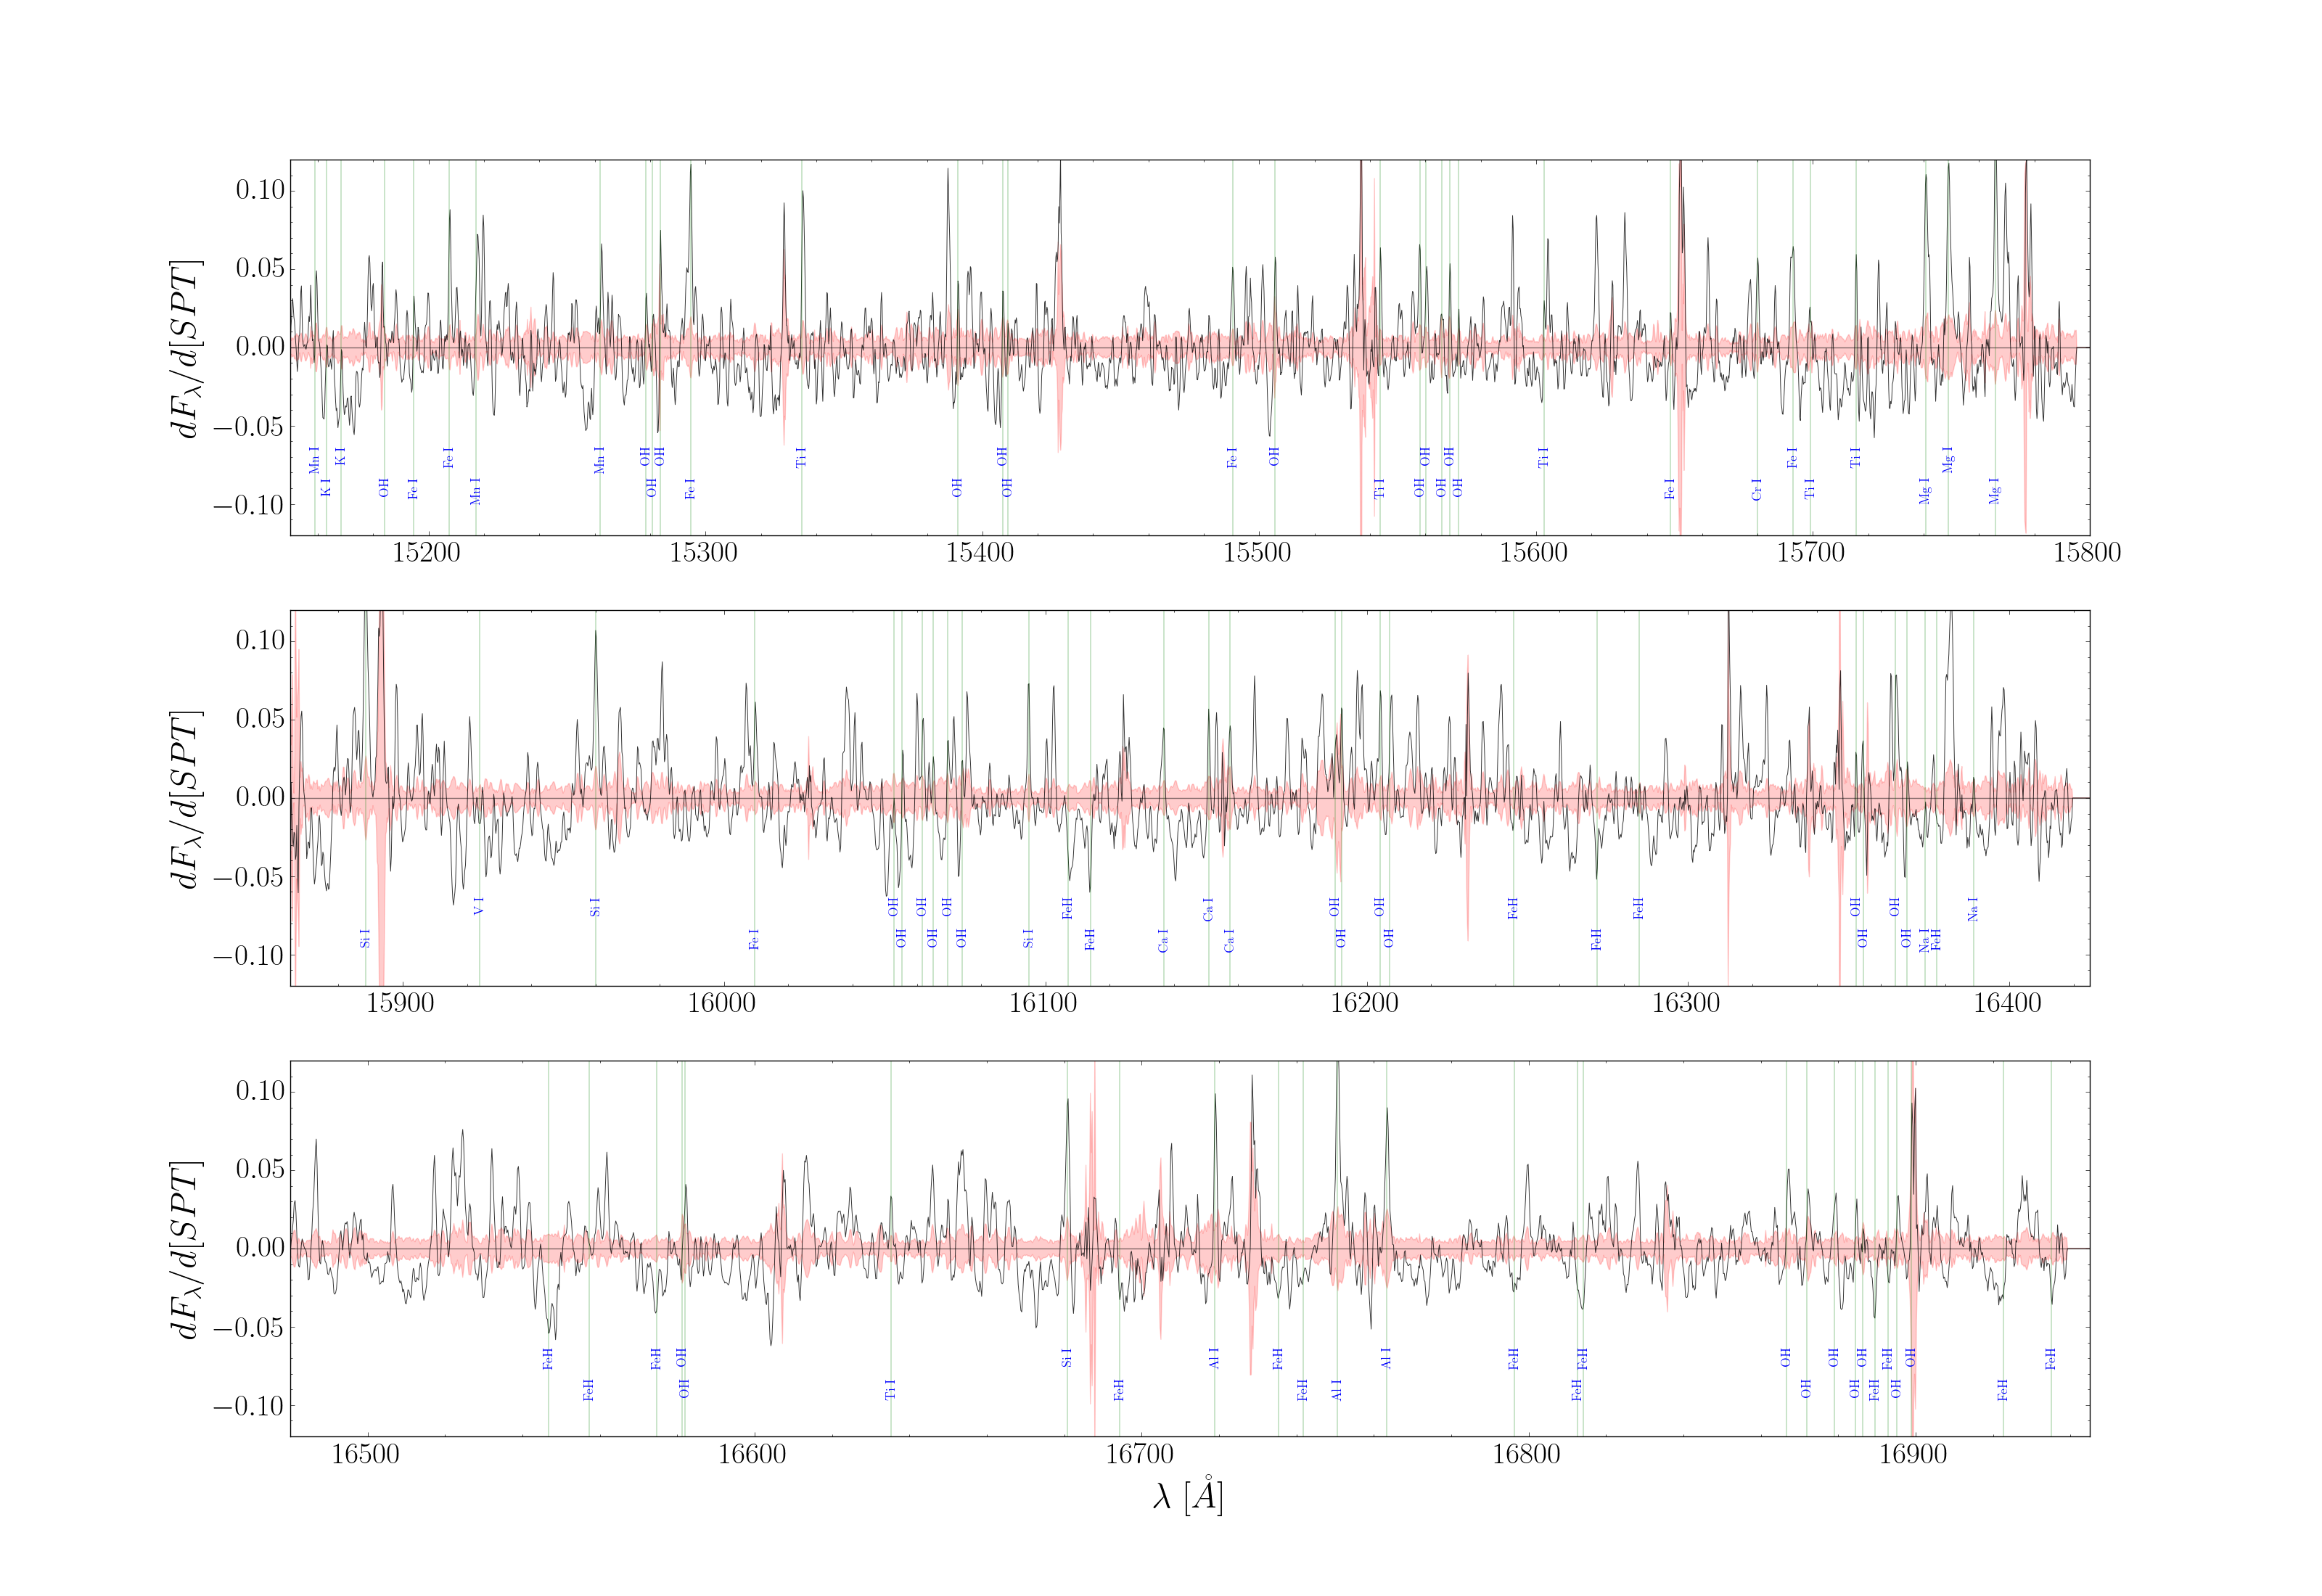
\includegraphics[width=16cm]{figures/derivative_jackknife_spt.png}
\end{center}
\caption{Derivative plots for spectral type model taken at the median training spectral type, SPT$=3$.} \label{fig:west_derivative}
\end{figure}

% \begin{figure}[ht]
% \begin{center}
% 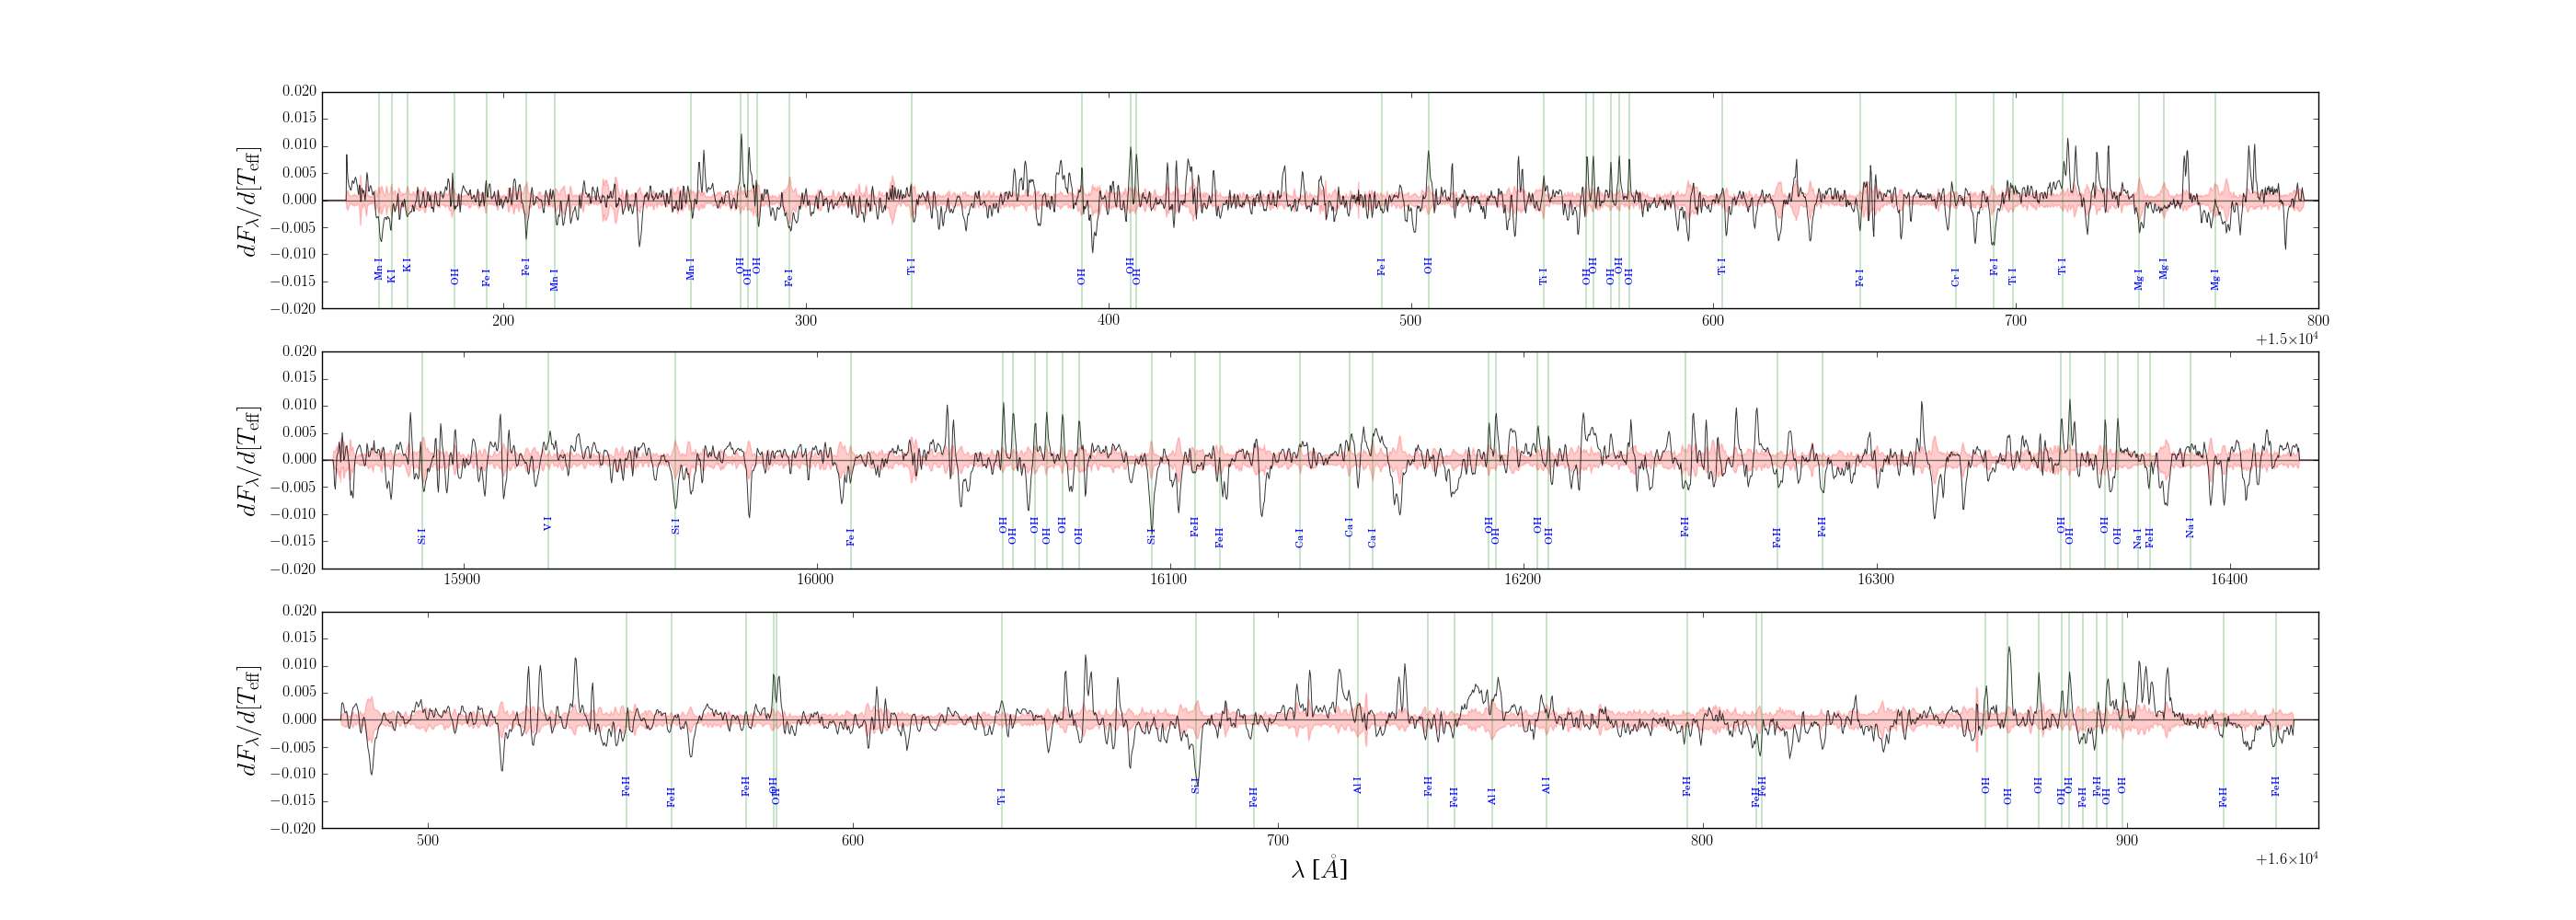
\includegraphics[width=16cm]{figures/derivative_jackknife_teff.png}
% 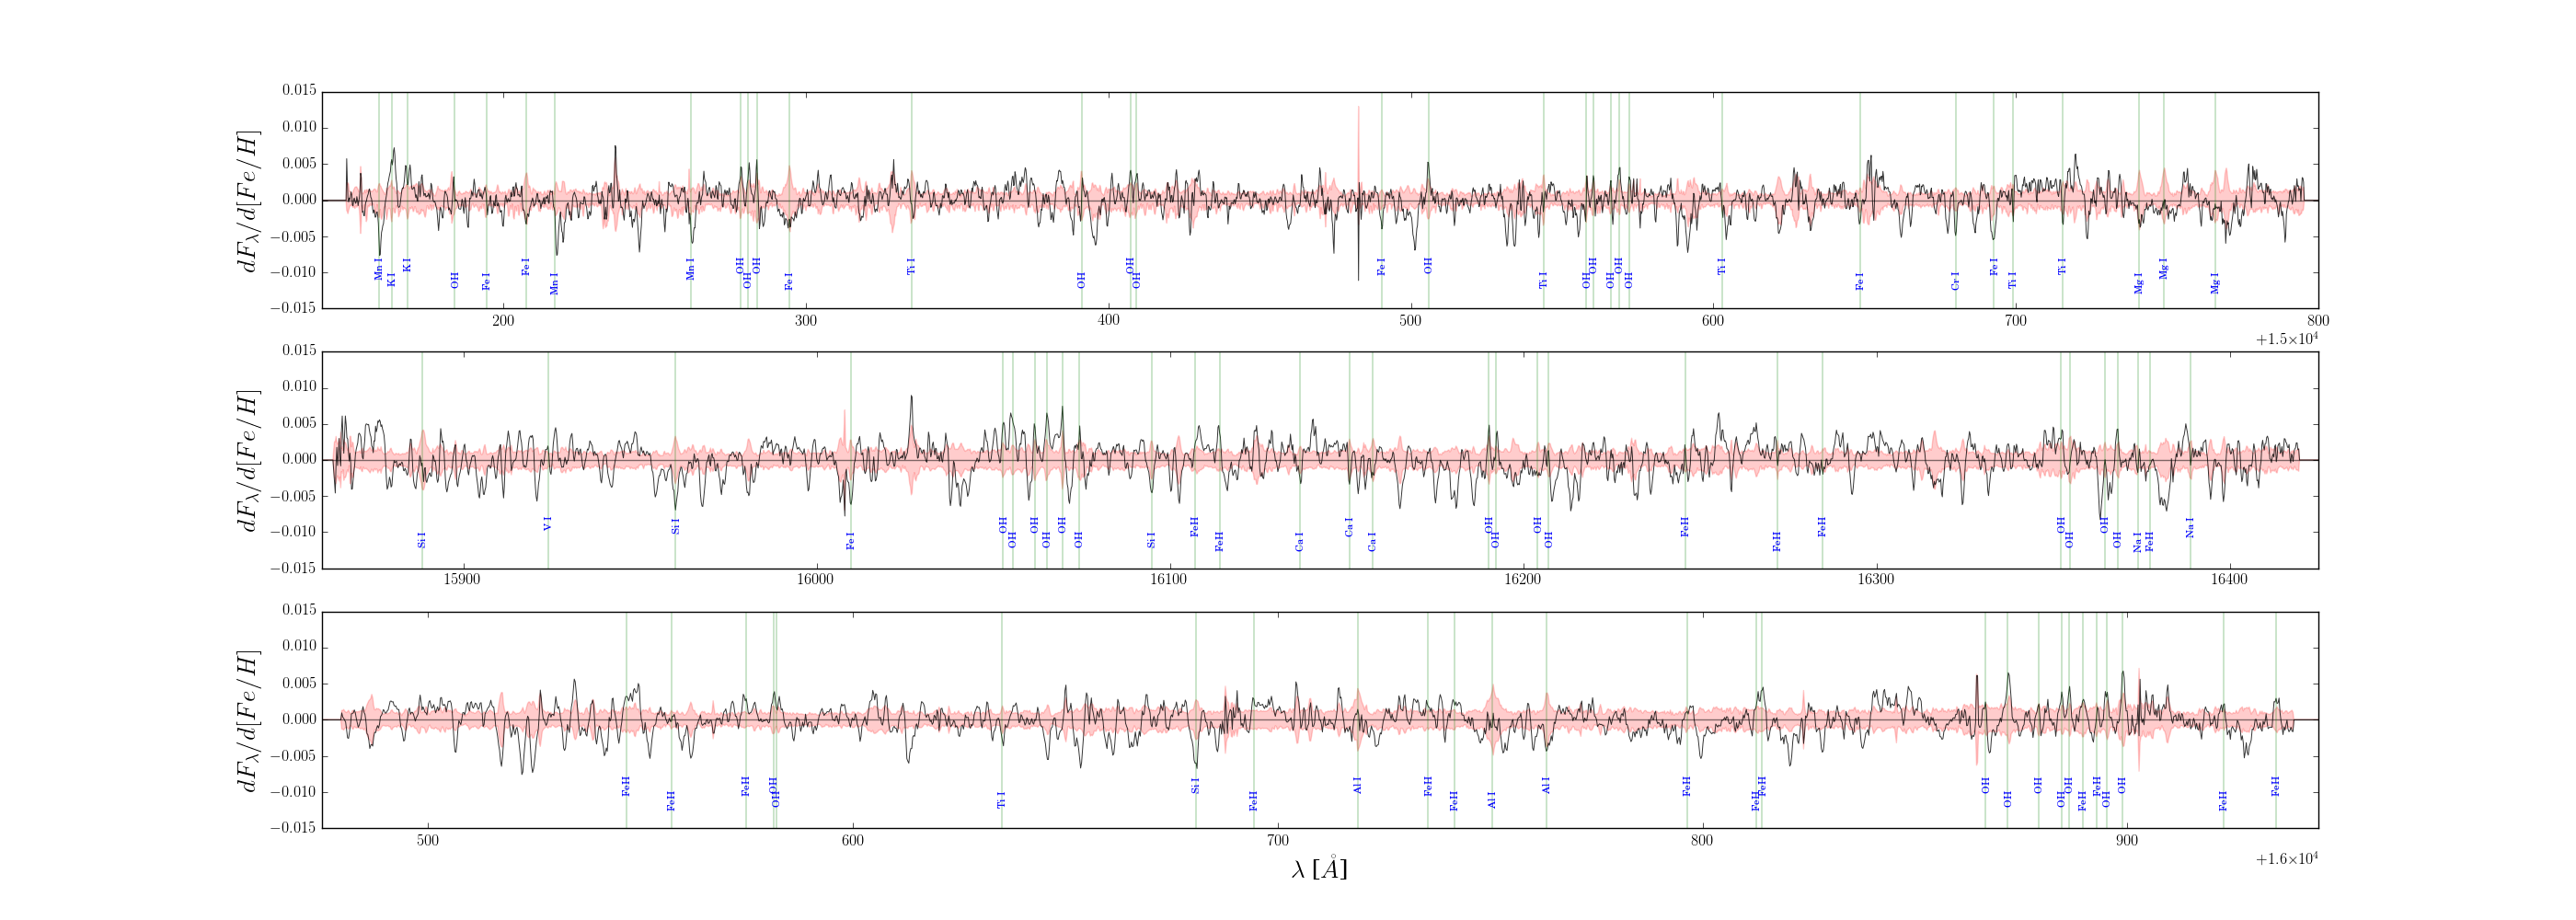
\includegraphics[width=16cm]{figures/derivative_jackknife_feh.png}
% \end{center}
% \caption{Derivative plots for physical parameter model. \textit{Top:} Derivative of flux with repsect to temperature taken at the median training temperature, T$_{\rm eff}=3463K$. \textit{Bottom:} Derivative of flux with repsect to metallicity taken at the median training metallicity, [Fe/H]$=-0.03$ dex.} \label{fig:mann_derivative}
% \end{figure}

\begin{figure}[ht]
\plotone{figures/cannon_chi_dist.png}
\caption{\textit{Left:} the distribution of fits for the training sample and known samples of pre-MS stars (\citealt{Cottaar:2014}) and binary sources (\citealt{ElBadry:2018}; \citealt{Skinner:2018}); \textit{right:} the distribution of $\chi^2$ fits for all 14,827 sources in the \apogee\-\gaia\ cross match, with color cuts $1<G_{BP}-G_{RP}<6$ and $7.5<M_{G}<20$ and $\pi>0$. We apply a quality cut of $\chi^2 < 100,000$ to the test sample for those sources we report as "safe". \label{fig:chi_dist}}
\end{figure}

\begin{figure}[ht]
\plotone{figures/cmd_selection.png}
\caption{\gaia\ and \zmass\ color-magnitude cuts for 12,037 sources with $\chi^2<100,000$. Over plotted with orange triangles are the 67 out of 87 training sample sources which have parallaxes measured by \gaia. \label{fig:cmd_selection}}
\end{figure}

\begin{figure}[ht]
\gridline{\fig{figures/safe_selection_teff.png}{0.5\textwidth}{}
          \fig{figures/safe_selection_feh.png}{0.5\textwidth}{}}
\gridline{\fig{figures/safe_selection_spt.png}{0.5\textwidth}{}}
\caption{Final sample selection with 10,311 M dwarfs based on criteria described in Section \ref{subsec:test_selection}. \label{fig:safe_selection}}
\end{figure}

\begin{figure}[ht]
\plotone{figures/spt_vs_teff_vs_feh.png}
\caption{West-trained spectral types vs. Mann-trained metallcities and temperatures. For each integer spectral type bin the mean temperatures and metallicities are shown as red error boxes. \label{fig:west_vs_mann}}
\end{figure}

\begin{figure}[ht]
\plotone{figures/aspcap_cannon_label_hist.png}
\caption{Distribution of temperatures and metallicities for 10,311 sources from \thecannon\ compared to the \aspcap\ pipeline. \label{fig:aspcap_cannon_label_hist}}
\end{figure}

%---------------------------
\begin{figure}[ht]
\plotone{figures/aspcap_cannon_validation.png}
\caption{Validation test \label{fig:aspcap_cannon_validation}}
\end{figure}


%%==========================================================================================
%% Tables

% \newpage 

\begin{longrotatetable}
\begin{deluxetable*}{ccc|ccc|ccc|c}
\tablecaption{Cannon results for Temperature/Metallicity model; see online journal for full table. \label{mann_results}}
\tabletypesize{\scriptsize}
\tablehead{
\multicolumn{3}{c}{\underline{Designation}} & \multicolumn{3}{c}{\underline{Temperature (K)}} & \multicolumn{3}{c}{\underline{Metallicity (dex)}} & \multicolumn{1}{c}{\underline{Model Fit}} \\
	  \colhead{2MASS ID} & \colhead{RA}   & \colhead{DEC}
    & \colhead{Training} & \colhead{Test} & \colhead{LOOCV}
    & \colhead{Training} & \colhead{Test} & \colhead{LOOCV} 
    & \colhead{Test $\chi^2$} 
} 
\startdata
2M00182256+4401222 & 4.59542   & 44.02278  & 3603        & 3538       & 3525        & -0.3       & -0.28     & -0.26      & 15304   \\
2M00182549+4401376 & 4.60779   & 44.02734  & 3218        & 3528       & 3560        & -0.3       & -0.29     & -0.29      & 21273   \\
2M00285391+5022330 & 7.22488   & 50.37588  & 3207        & 3190       & 3192        & 0.11       & 0.04      & 0.01       & 31790   \\
2M00401001+0308050 & 10.04169  & 3.13473   & 3725        & 3777       & 3772        & 0.04       & 0.12      & 0.14       & 9830    \\
2M00580115+3919111 & 14.50482  & 39.31977  & 3157        & 3100       & 3107        & -0.07      & -0.02     & 0.01       & 13337   \\
2M01232542+1638384 & 20.8559   & 16.64401  & 3272        & 3225       & 3223        & 0.1        & 0.02      & -0.01      & 34797   \\
2M02001278+1303112 & 30.05402  & 13.05196  & 3080        & 3059       & 3077        & -0.16      & -0.1      & -0.02      & 33210   \\
2M02361535+0652191 & 39.06358  & 6.87167   & 3284        & 3241       & 3243        & -0.12      & -0.28     & -0.28      & 48445   \\
2M03044335+6144097 & 46.18104  & 61.73583  & 3500        & 3466       & 3466        & -0.12      & -0.26     & -0.28      & 40739   \\
2M03553688+5214291 & 58.90373  & 52.2414   & 3435        & 3386       & 3375        & -0.35      & -0.28     & -0.2       & 53870   \\
2M04125880+5236421 & 63.24499  & 52.61165  & 3100        & 3183       & 3204        & -0.04      & -0.01     & 0.0        & 46007   \\
2M04310001+3647548 & 67.75003  & 36.79855  & 3419        & 3371       & 3369        & 0.08       & 0.11      & 0.1        & 20602   \\
2M05222053+3031097 & 80.58561  & 30.51933  & 3389        & 3423       & 3431        & 0.28       & 0.18      & 0.13       & 19072   \\
2M05312734-0340356 & 82.86417  & -3.67722  & 3801        & 3814       & 3849        & 0.49       & 0.5       & 0.36       & 28209   \\
2M05413073+5329239 & 85.37804  & 53.48987  & 3765        & 3751       & 3753        & 0.19       & 0.15      & 0.14       & 17842   \\
2M05420897+1229252 & 85.53833  & 12.48956  & 3250        & 3220       & 3229        & -0.22      & -0.33     & -0.29      & 33868   \\
2M06000351+0242236 & 90.01458  & 2.70657   & 3214        & 3170       & 3170        & 0.07       & 0.03      & 0.01       & 21044   \\
2M06011106+5935508 & 90.2961   & 59.59713  & 3340        & 3259       & 3255        & -0.09      & -0.05     & -0.04      & 23329   \\
2M06112610+1032599 & 92.8588   & 10.54998  & 3636        & 3720       & 3706        & -0.39      & -0.43     & -0.4       & 36898   \\
2M06544902+3316058 & 103.70411 & 33.26823  & 3448        & 3368       & 3363        & -0.02      & 0.03      & 0.04       & 19412   \\
2M07171706-0501031 & 109.32108 & -5.01754  & 3193        & 3175       & 3188        & -0.09      & -0.15     & -0.13      & 103000  \\
2M07272450+0513329 & 111.852   & 5.2263    & 3317        & 3279       & 3279        & -0.11      & -0.18     & -0.17      & 23615   \\
2M07444018+0333089 & 116.16744 & 3.55252   & 3217        & 3174       & 3167        & 0.23       & 0.25      & 0.17       & 34181   \\
2M08031949+5250387 & 120.83131 & 52.84402  & 3508        & 3617       & 3620        & -0.26      & -0.23     & -0.23      & 17491   \\
\nodata & \nodata & \nodata & \nodata & \nodata & \nodata & \nodata & \nodata & \nodata & \nodata
\enddata
\end{deluxetable*}
\end{longrotatetable}

%====================================
\newpage 

\begin{longrotatetable}
\begin{deluxetable*}{ccc|ccc|c}
\tablecaption{Cannon results for Spectral Type model. \label{west_results}}
\tabletypesize{\scriptsize}
\tablehead{
\multicolumn{3}{c}{\underline{Designation}} & \multicolumn{3}{c}{\underline{Spectral Type}}
	& \multicolumn{1}{c}{\underline{Model Fit}} \\
	  \colhead{2MASS ID} & \colhead{RA}   & \colhead{DEC}
    & \colhead{Training} & \colhead{Test} & \colhead{LOOCV} 
    & \colhead{Test $\chi^2$}
} 
\startdata
2M03114974+0115158 & 47.957262  & 1.254404  & 1          & 0.9       & 1.4        & 78236   \\
2M03122509+0021585 & 48.104563  & 0.366251  & 7          & 7.3       & 5.5        & 56504   \\
2M03423963+0012102 & 55.66513   & 0.202859  & 4          & 3.9       & 3.9        & 29598   \\
2M04262170+1800009 & 66.590421  & 18.000265 & 5          & 5.0       & 5.1        & 14084   \\
2M09152918+4407461 & 138.871602 & 44.129498 & 3          & 3.6       & 3.7        & 17921   \\
2M09183649+2207022 & 139.652051 & 22.117298 & 3          & 2.4       & 2.4        & 10591   \\
2M09332262+2749021 & 143.344279 & 27.817253 & 3          & 2.8       & 2.7        & 17388   \\
2M09373349+5534057 & 144.389577 & 55.568275 & 6          & 6.5       & 6.4        & 15335   \\
2M10313413+3441535 & 157.892222 & 34.698212 & 1          & 2.0       & 2.3        & 21134   \\
2M11194647+0820356 & 169.943658 & 8.343246  & 8          & 7.5       & 6.5        & 37803   \\
2M11203609+0704135 & 170.1504   & 7.070432  & 6          & 6.1       & 5.9        & 18677   \\
2M11570299+2028436 & 179.262465 & 20.4788   & 2          & 2.9       & 3.0        & 16205   \\
2M12203634+2505351 & 185.15143  & 25.093107 & 4          & 3.4       & 3.1        & 85745   \\
2M12212701-0030560 & 185.362567 & -0.515566 & 0          & 1.4       & 1.8        & 22646   \\
2M12423245-0646077 & 190.635249 & -6.768827 & 2          & 2.4       & 2.5        & 18410   \\
2M12464541-0312524 & 191.689212 & -3.214578 & 4          & 3.6       & 3.5        & 11561   \\
2M12471099+1109566 & 191.795795 & 11.165737 & 3          & 3.1       & 3.0        & 12738   \\
2M12492657-0312032 & 192.360749 & -3.200903 & 3          & 3.3       & 3.5        & 37756   \\
2M12503440+4309482 & 192.643353 & 43.163414 & 4          & 4.0       & 4.0        & 19726   \\
2M12523816+1240586 & 193.159002 & 12.682945 & 4          & 4.1       & 4.1        & 15526   \\
2M12552141+4150425 & 193.839213 & 41.845161 & 3          & 3.1       & 3.1        & 29274   \\
2M12564117+4233175 & 194.171558 & 42.554871 & 3          & 3.1       & 3.1        & 35083   \\
2M13032161+4220407 & 195.840051 & 42.344654 & 2          & 2.7       & 2.8        & 14657   \\
2M13415860+1852278 & 205.494169 & 18.874393 & 4          & 3.9       & 3.9        & 9475    \\
2M13442970+5625445 & 206.123779 & 56.429039 & 5          & 5.9       & 6.0        & 16017   \\
\nodata & \nodata & \nodata & \nodata & \nodata & \nodata & \nodata
\enddata
\end{deluxetable*}
\end{longrotatetable}

%====================================
\newpage 


%%==========================================================================================
\clearpage
\bibliographystyle{aasjournal}
\bibliography{ref}

\end{document}


